% Options for packages loaded elsewhere
\PassOptionsToPackage{unicode}{hyperref}
\PassOptionsToPackage{hyphens}{url}
\PassOptionsToPackage{dvipsnames,svgnames,x11names}{xcolor}
%
\documentclass[
  letterpaper,
  DIV=11,
  numbers=noendperiod]{scrartcl}

\usepackage{amsmath,amssymb}
\usepackage{iftex}
\ifPDFTeX
  \usepackage[T1]{fontenc}
  \usepackage[utf8]{inputenc}
  \usepackage{textcomp} % provide euro and other symbols
\else % if luatex or xetex
  \usepackage{unicode-math}
  \defaultfontfeatures{Scale=MatchLowercase}
  \defaultfontfeatures[\rmfamily]{Ligatures=TeX,Scale=1}
\fi
\usepackage{lmodern}
\ifPDFTeX\else  
    % xetex/luatex font selection
\fi
% Use upquote if available, for straight quotes in verbatim environments
\IfFileExists{upquote.sty}{\usepackage{upquote}}{}
\IfFileExists{microtype.sty}{% use microtype if available
  \usepackage[]{microtype}
  \UseMicrotypeSet[protrusion]{basicmath} % disable protrusion for tt fonts
}{}
\makeatletter
\@ifundefined{KOMAClassName}{% if non-KOMA class
  \IfFileExists{parskip.sty}{%
    \usepackage{parskip}
  }{% else
    \setlength{\parindent}{0pt}
    \setlength{\parskip}{6pt plus 2pt minus 1pt}}
}{% if KOMA class
  \KOMAoptions{parskip=half}}
\makeatother
\usepackage{xcolor}
\setlength{\emergencystretch}{3em} % prevent overfull lines
\setcounter{secnumdepth}{-\maxdimen} % remove section numbering
% Make \paragraph and \subparagraph free-standing
\makeatletter
\ifx\paragraph\undefined\else
  \let\oldparagraph\paragraph
  \renewcommand{\paragraph}{
    \@ifstar
      \xxxParagraphStar
      \xxxParagraphNoStar
  }
  \newcommand{\xxxParagraphStar}[1]{\oldparagraph*{#1}\mbox{}}
  \newcommand{\xxxParagraphNoStar}[1]{\oldparagraph{#1}\mbox{}}
\fi
\ifx\subparagraph\undefined\else
  \let\oldsubparagraph\subparagraph
  \renewcommand{\subparagraph}{
    \@ifstar
      \xxxSubParagraphStar
      \xxxSubParagraphNoStar
  }
  \newcommand{\xxxSubParagraphStar}[1]{\oldsubparagraph*{#1}\mbox{}}
  \newcommand{\xxxSubParagraphNoStar}[1]{\oldsubparagraph{#1}\mbox{}}
\fi
\makeatother


\providecommand{\tightlist}{%
  \setlength{\itemsep}{0pt}\setlength{\parskip}{0pt}}\usepackage{longtable,booktabs,array}
\usepackage{calc} % for calculating minipage widths
% Correct order of tables after \paragraph or \subparagraph
\usepackage{etoolbox}
\makeatletter
\patchcmd\longtable{\par}{\if@noskipsec\mbox{}\fi\par}{}{}
\makeatother
% Allow footnotes in longtable head/foot
\IfFileExists{footnotehyper.sty}{\usepackage{footnotehyper}}{\usepackage{footnote}}
\makesavenoteenv{longtable}
\usepackage{graphicx}
\makeatletter
\def\maxwidth{\ifdim\Gin@nat@width>\linewidth\linewidth\else\Gin@nat@width\fi}
\def\maxheight{\ifdim\Gin@nat@height>\textheight\textheight\else\Gin@nat@height\fi}
\makeatother
% Scale images if necessary, so that they will not overflow the page
% margins by default, and it is still possible to overwrite the defaults
% using explicit options in \includegraphics[width, height, ...]{}
\setkeys{Gin}{width=\maxwidth,height=\maxheight,keepaspectratio}
% Set default figure placement to htbp
\makeatletter
\def\fps@figure{htbp}
\makeatother

\usepackage{booktabs}
\usepackage{longtable}
\usepackage{array}
\usepackage{multirow}
\usepackage{wrapfig}
\usepackage{float}
\usepackage{colortbl}
\usepackage{pdflscape}
\usepackage{tabu}
\usepackage{threeparttable}
\usepackage{threeparttablex}
\usepackage[normalem]{ulem}
\usepackage{makecell}
\usepackage{xcolor}
\usepackage{booktabs}
\usepackage{longtable}
\KOMAoption{captions}{tableheading}
\makeatletter
\@ifpackageloaded{caption}{}{\usepackage{caption}}
\AtBeginDocument{%
\ifdefined\contentsname
  \renewcommand*\contentsname{Table of contents}
\else
  \newcommand\contentsname{Table of contents}
\fi
\ifdefined\listfigurename
  \renewcommand*\listfigurename{List of Figures}
\else
  \newcommand\listfigurename{List of Figures}
\fi
\ifdefined\listtablename
  \renewcommand*\listtablename{List of Tables}
\else
  \newcommand\listtablename{List of Tables}
\fi
\ifdefined\figurename
  \renewcommand*\figurename{Figure}
\else
  \newcommand\figurename{Figure}
\fi
\ifdefined\tablename
  \renewcommand*\tablename{Table}
\else
  \newcommand\tablename{Table}
\fi
}
\@ifpackageloaded{float}{}{\usepackage{float}}
\floatstyle{ruled}
\@ifundefined{c@chapter}{\newfloat{codelisting}{h}{lop}}{\newfloat{codelisting}{h}{lop}[chapter]}
\floatname{codelisting}{Listing}
\newcommand*\listoflistings{\listof{codelisting}{List of Listings}}
\makeatother
\makeatletter
\makeatother
\makeatletter
\@ifpackageloaded{caption}{}{\usepackage{caption}}
\@ifpackageloaded{subcaption}{}{\usepackage{subcaption}}
\makeatother

\ifLuaTeX
  \usepackage{selnolig}  % disable illegal ligatures
\fi
\usepackage{bookmark}

\IfFileExists{xurl.sty}{\usepackage{xurl}}{} % add URL line breaks if available
\urlstyle{same} % disable monospaced font for URLs
\hypersetup{
  pdftitle={DAA Metacyc},
  colorlinks=true,
  linkcolor={blue},
  filecolor={Maroon},
  citecolor={Blue},
  urlcolor={Blue},
  pdfcreator={LaTeX via pandoc}}


\title{DAA Metacyc}
\author{}
\date{}

\begin{document}
\maketitle


\subsubsection{Differential abundance
analysis}\label{differential-abundance-analysis}

\begin{itemize}
\tightlist
\item
  Group variable: \textbf{diet}
\item
  Formula used: \textbf{\textasciitilde{} diet * time + (1 \textbar{}
  id)}
\end{itemize}

\begin{longtable}[t]{lrrrrrr}
\caption{Table of significant features}\\
\toprule
\textbf{feature} & \textbf{metadata} & \textbf{value} & \textbf{coef} & \textbf{qval\_individual} & \textbf{qval\_joint} & \textbf{model}\\
\midrule
\endfirsthead
\caption[]{Table of significant features \textit{(continued)}}\\
\toprule
\textbf{feature} & \textbf{metadata} & \textbf{value} & \textbf{coef} & \textbf{qval\_individual} & \textbf{qval\_joint} & \textbf{model}\\
\midrule
\endhead

\endfoot
\bottomrule
\endlastfoot
X5.1.99.... & time & time & -10.602 & 0.000 & 0.000 & prevalence\\
X5.1.99.... & diet & 2 & -20.311 & 0.001 & 0.001 & prevalence\\
X5.1.99.... & diet & 2:time & 10.603 & 0.002 & 0.003 & prevalence\\
X4.2.2.2 & diet & 2:time & -2.360 & 0.007 & 0.009 & abundance\\
X2.3.1.2... & diet & 2:time & -0.778 & 0.021 & 0.018 & abundance\\
\addlinespace
X2.3.3.1... & diet & 2 & 6.922 & 0.021 & 0.023 & abundance\\
X1.1.1.1... & time & time & 10.079 & 0.021 & 0.018 & prevalence\\
X3.6.3.5 & diet & 2 & -2.369 & 0.038 & 0.027 & abundance\\
X3.1.1.8... & time & time & -0.862 & 0.050 & 0.036 & abundance\\
X4.2.2.2 & diet & 2 & 3.165 & 0.058 & 0.059 & abundance\\
\addlinespace
X1.2.1.6... & time & time & -1.857 & 0.060 & 0.047 & abundance\\
X4.2.1.1... & diet & 2:time & -0.885 & 0.060 & 0.047 & abundance\\
X3.1.1.7... & diet & 2:time & -2.355 & 0.063 & 0.048 & abundance\\
X2.1.1.1... & diet & 2:time & -1.913 & 0.070 & 0.091 & abundance\\
X2.3.3.1... & diet & 2:time & -3.639 & 0.070 & 0.091 & abundance\\
\addlinespace
X3.6.3.5 & diet & 2:time & 1.380 & 0.070 & 0.059 & abundance\\
X4.2.1.1... & diet & 2:time & 2.345 & 0.070 & 0.091 & abundance\\
X2.1.1.1... & diet & 2 & 3.104 & 0.070 & 0.091 & abundance\\
X2.1.1.1... & diet & 2:time & 10.416 & 0.070 & 0.091 & prevalence\\
X2.4.1.2... & diet & 2 & -8.348 & 0.070 & 0.091 & prevalence\\
\addlinespace
X2.8.3.1... & diet & 2:time & 11.176 & 0.073 & 0.095 & prevalence\\
X2.3.1.2... & diet & 2 & 1.017 & 0.103 & 0.091 & abundance\\
X5.1.1.1... & diet & 2 & -1.887 & 0.103 & 0.091 & abundance\\
X2.3.3.1... & diet & 2:time & 1.252 & 0.671 & 0.091 & prevalence\\
X2.8.3.1... & diet & 2:time & -1.960 & 0.694 & 0.095 & abundance\\
\addlinespace
X2.3.3.1... & diet & 2 & -1.731 & 0.759 & 0.023 & prevalence\\
X5.1.99.... & diet & 2:time & -0.498 & 0.791 & 0.003 & abundance\\
X5.1.99.... & diet & 2 & 0.704 & 0.826 & 0.001 & abundance\\
X2.1.1.1... & diet & 2:time & 0.628 & 0.880 & 0.091 & abundance\\
X4.2.2.2 & diet & 2 & -3.784 & 0.898 & 0.059 & prevalence\\
\addlinespace
X2.1.1.1... & diet & 2 & -3.229 & 0.917 & 0.091 & prevalence\\
X5.1.99.... & time & time & -0.191 & 0.931 & 0.000 & abundance\\
X4.2.2.2 & diet & 2:time & 1.892 & 0.945 & 0.009 & prevalence\\
X2.1.1.1... & diet & 2:time & 0.956 & 0.997 & 0.091 & prevalence\\
X2.4.1.2... & diet & 2 & -0.076 & 1.000 & 0.091 & abundance\\
\addlinespace
X4.2.1.1... & diet & 2:time & 9.941 & 1.000 & 0.091 & prevalence\\
X1.2.1.6... & time & time & 0.000 & 1.000 & 0.047 & prevalence\\
X1.1.1.1... & time & time & -1.281 & NA & 0.018 & abundance\\
X2.3.1.2... & diet & 2 & NA & NA & 0.091 & prevalence\\
X2.3.1.2... & diet & 2:time & NA & NA & 0.018 & prevalence\\
\addlinespace
X3.1.1.7... & diet & 2:time & 20.630 & NA & 0.048 & prevalence\\
X3.1.1.8... & time & time & NA & NA & 0.036 & prevalence\\
X3.6.3.5 & diet & 2 & NA & NA & 0.027 & prevalence\\
X3.6.3.5 & diet & 2:time & NA & NA & 0.059 & prevalence\\
X4.2.1.1... & diet & 2:time & NA & NA & 0.047 & prevalence\\
\addlinespace
X5.1.1.1... & diet & 2 & NA & NA & 0.091 & prevalence\\*
\end{longtable}

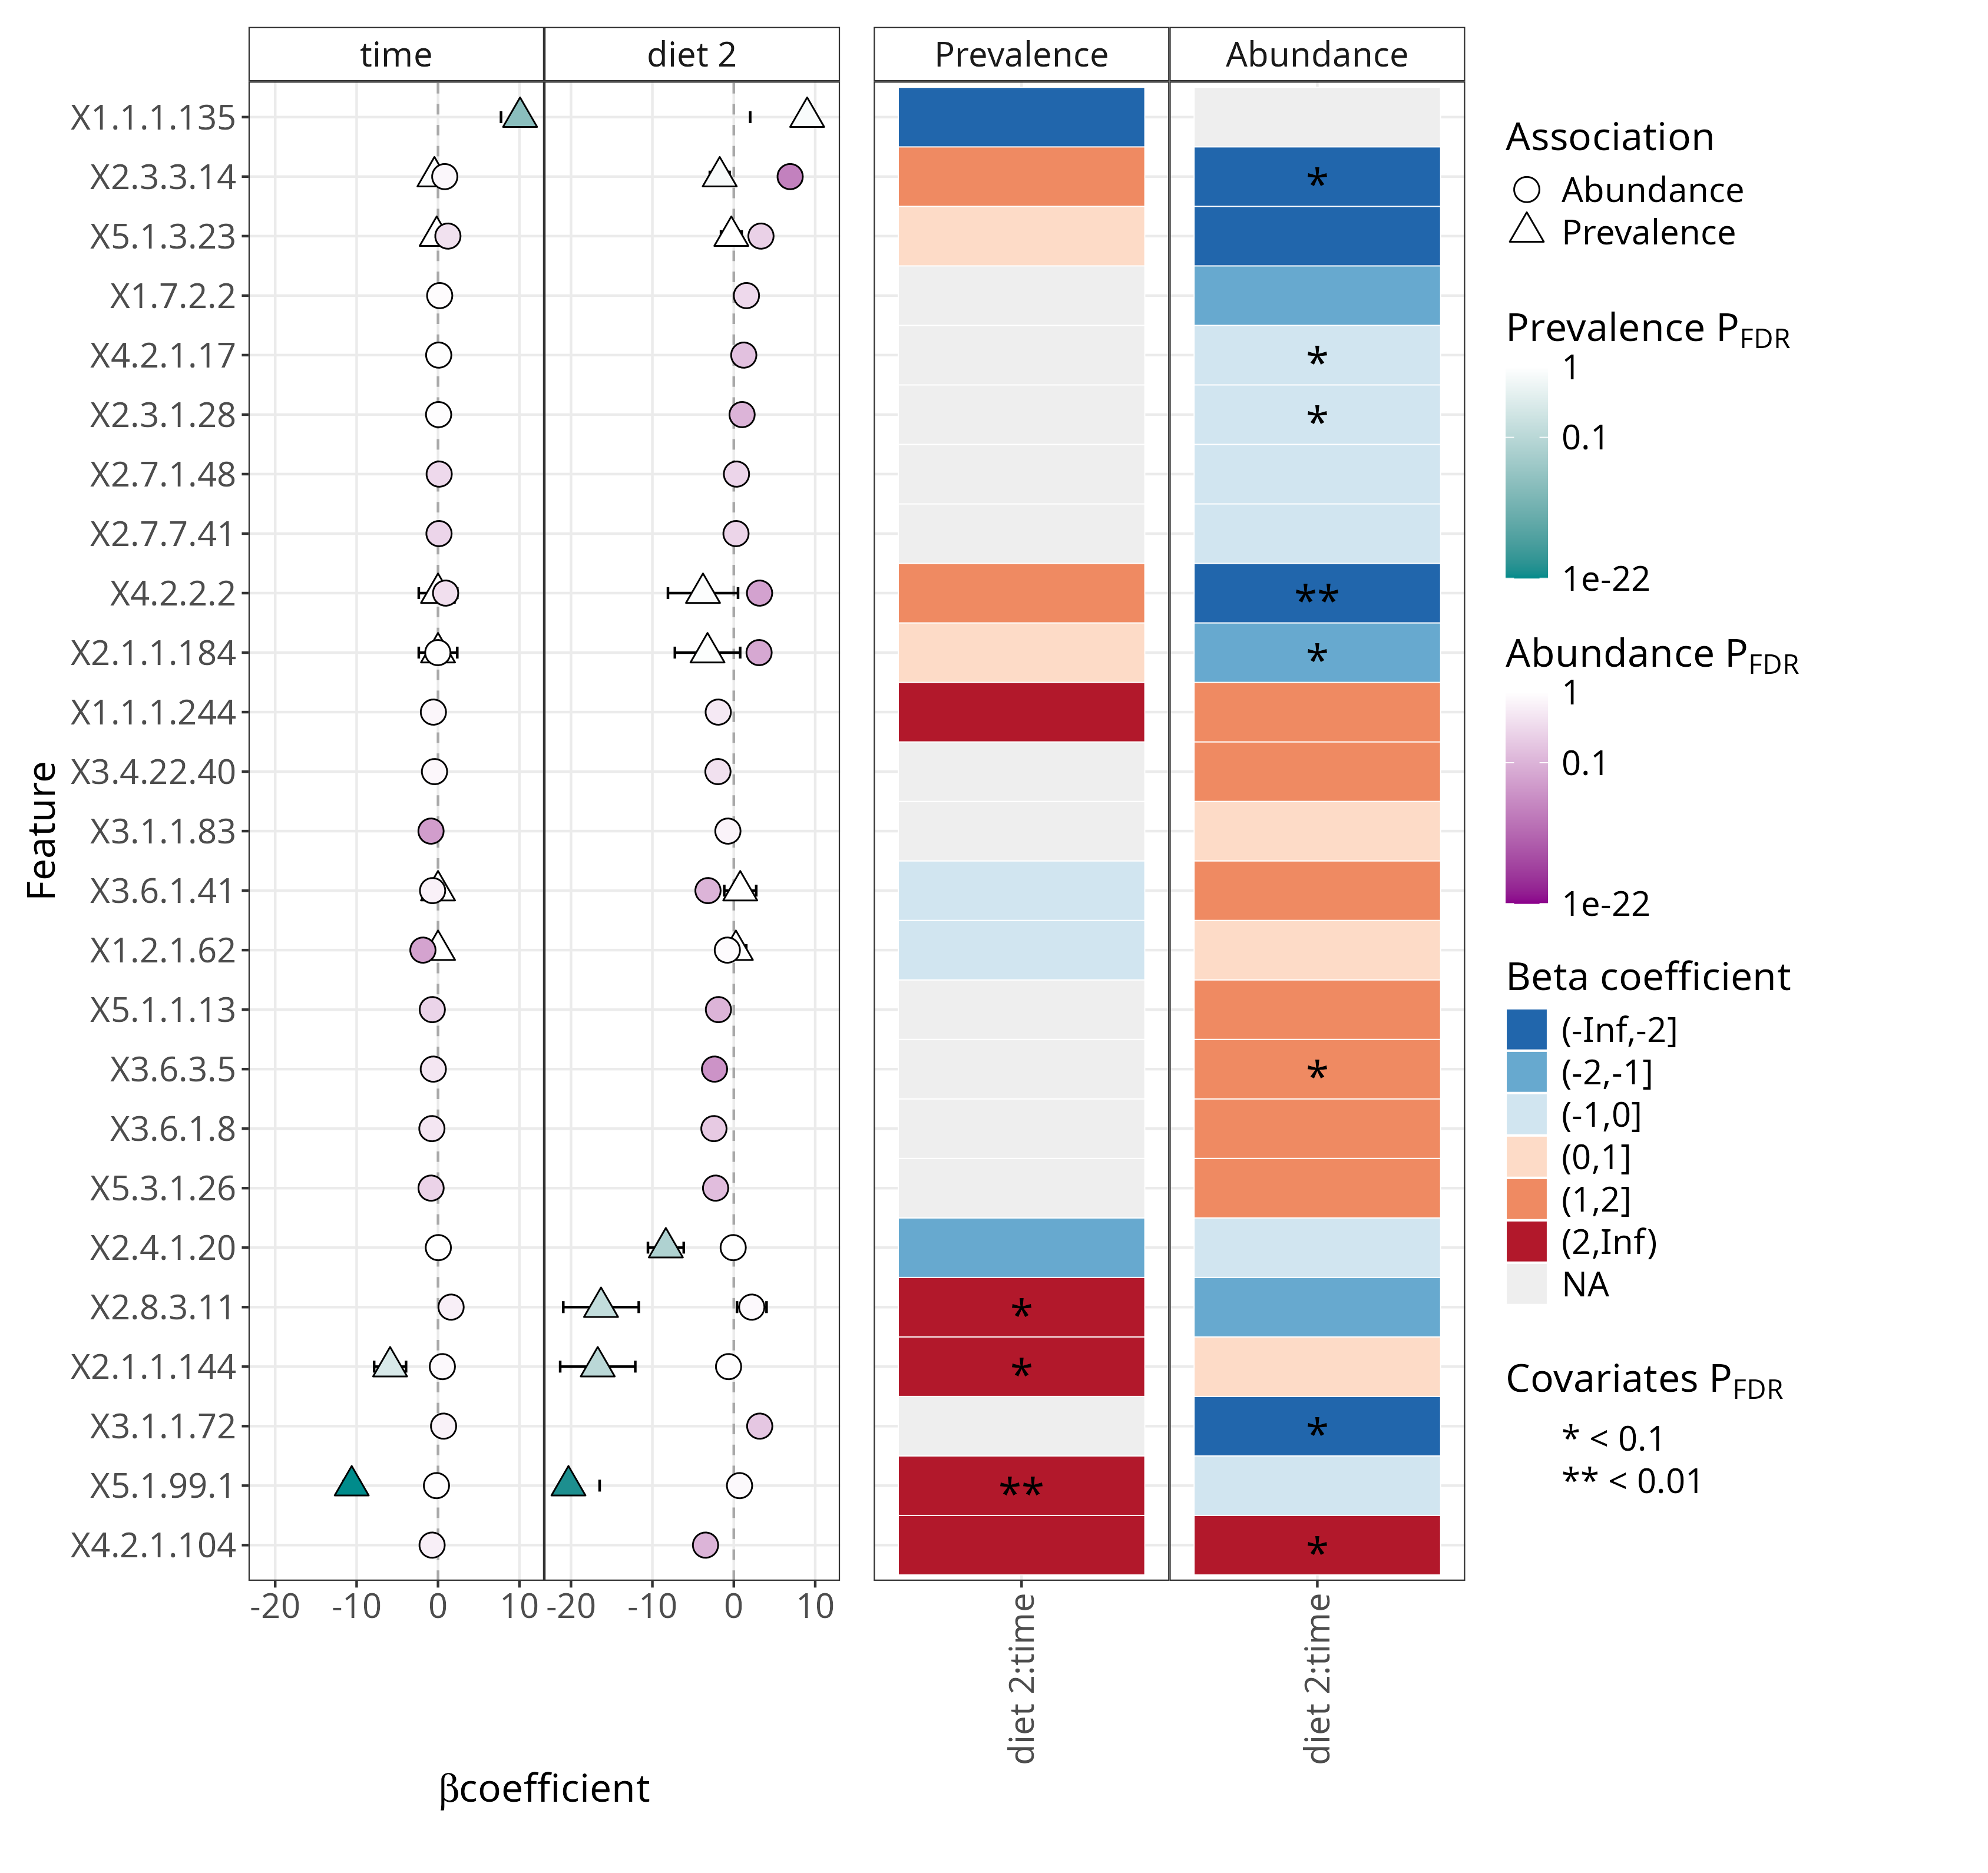
\includegraphics{../output/daa/daa_mtc/figures/summary_plot.png}
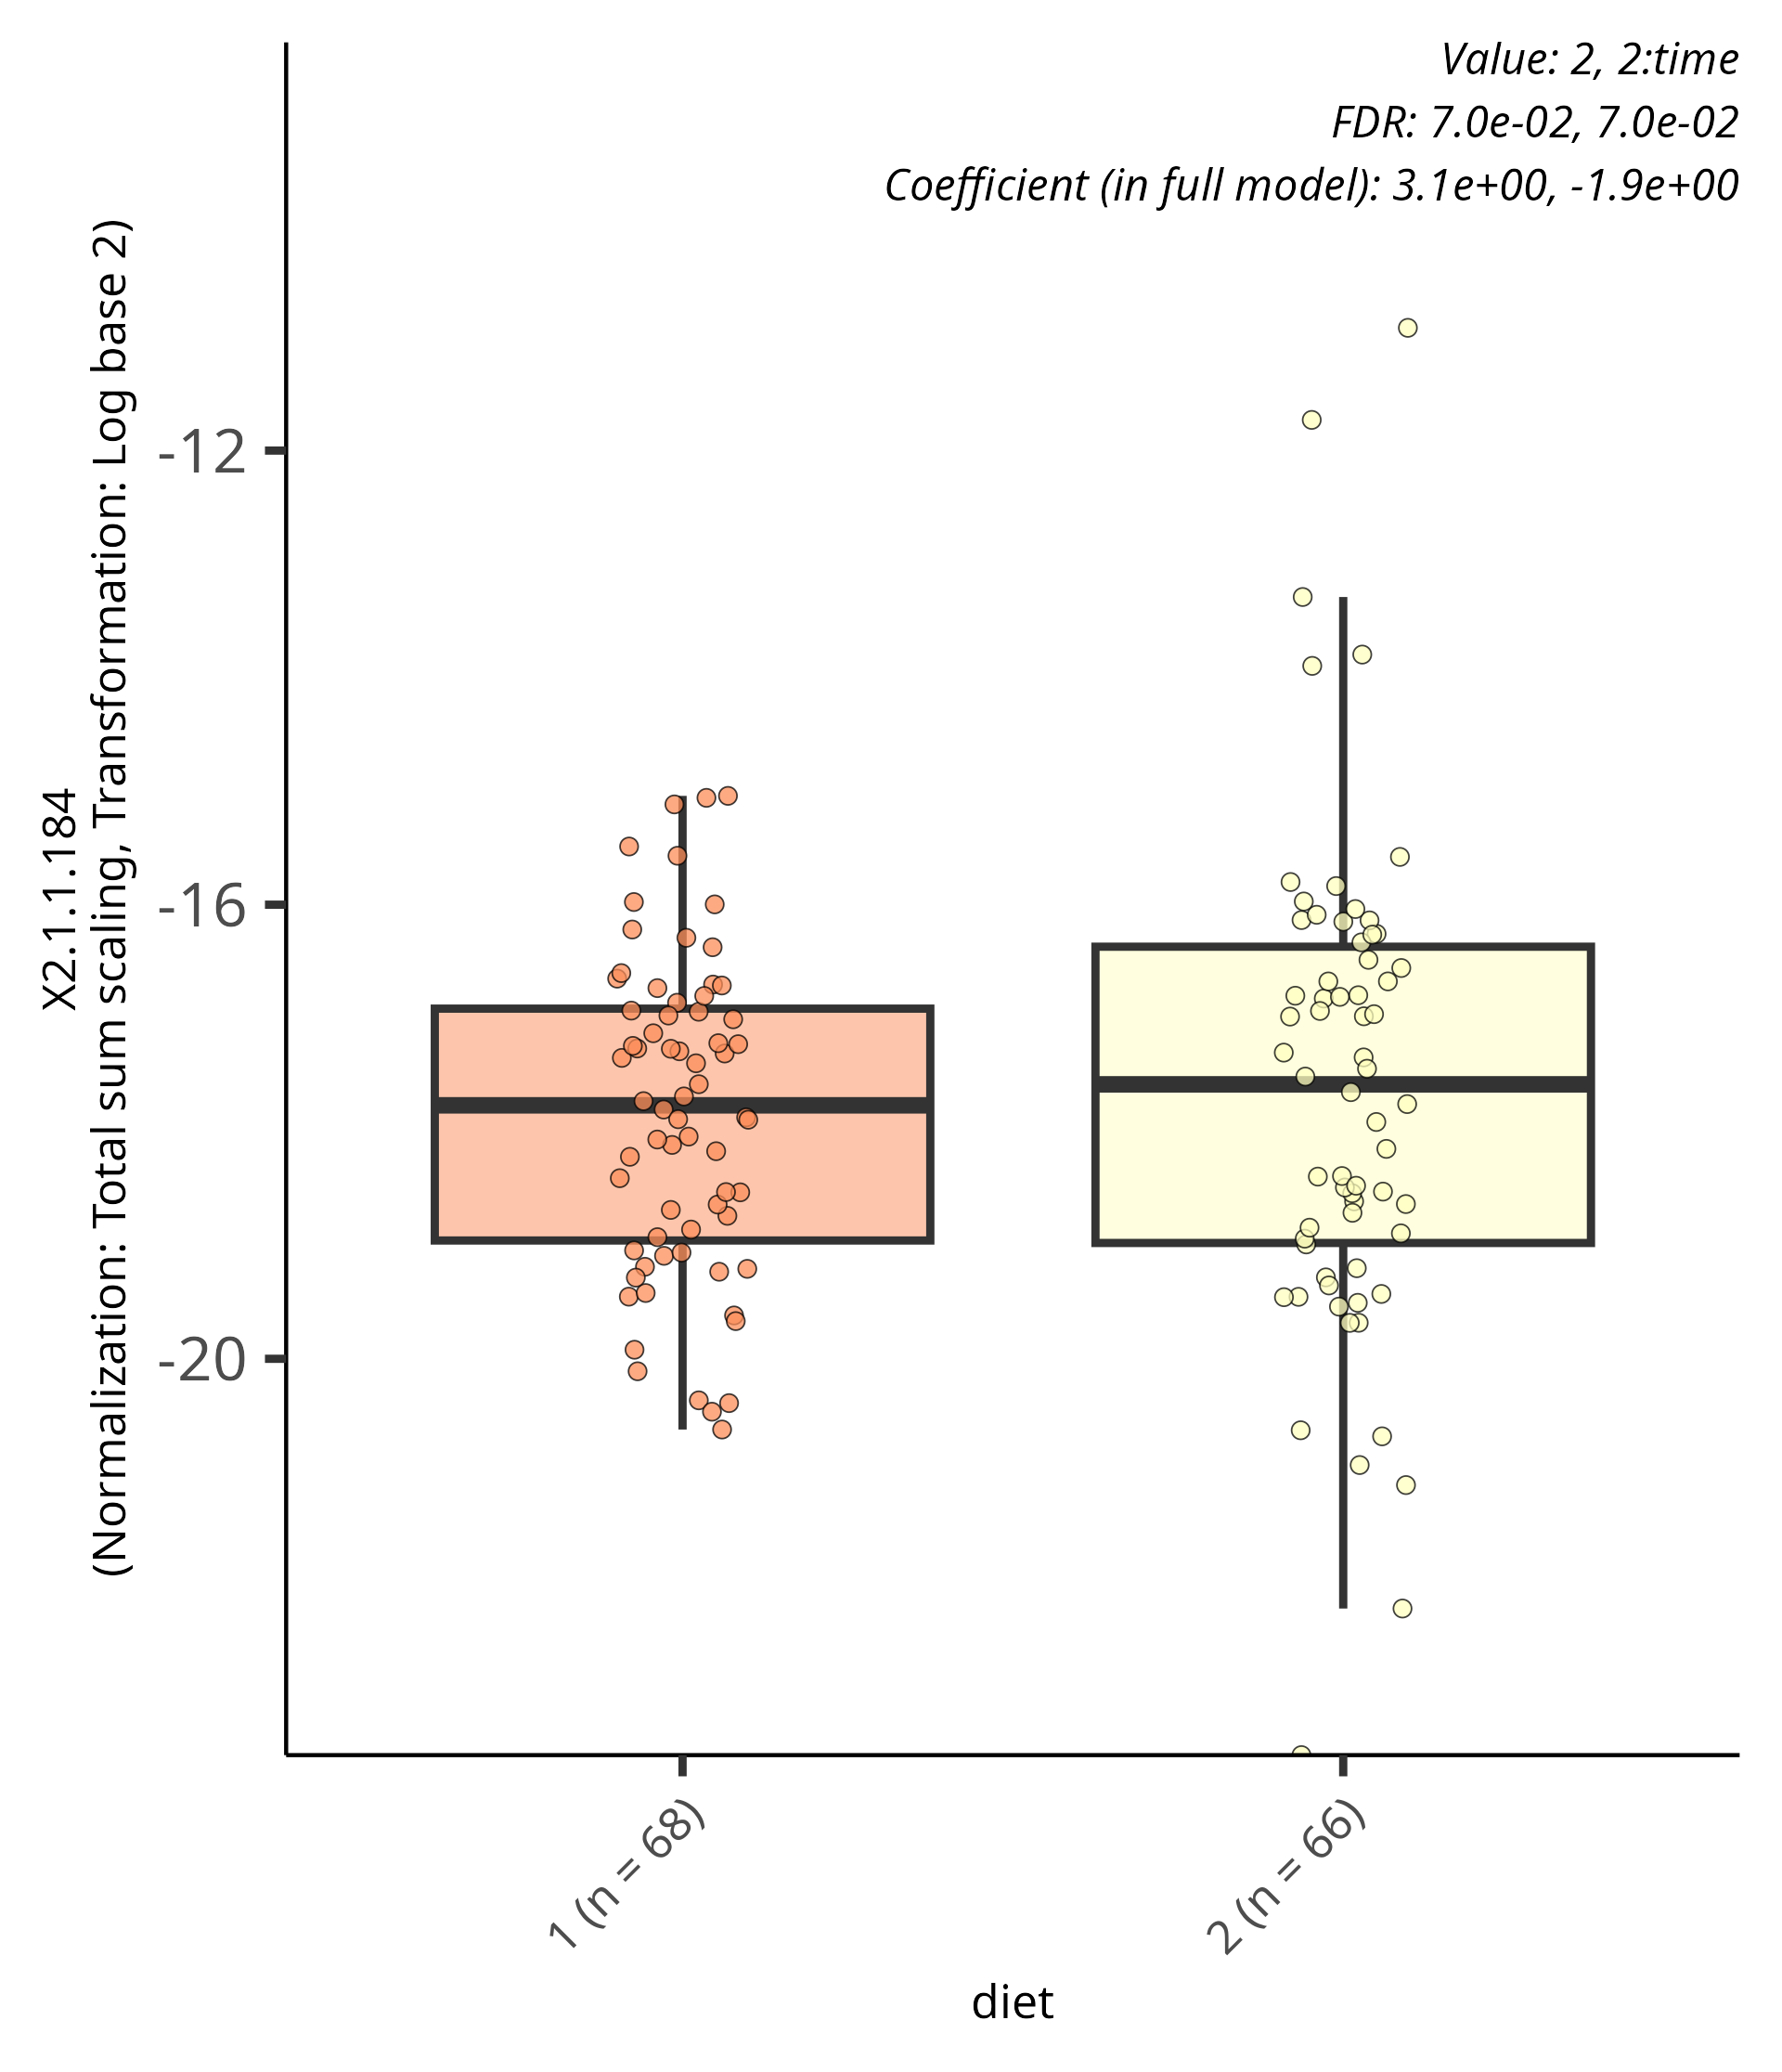
\includegraphics{../output/daa/daa_mtc/figures/association_plots/diet/linear/diet_X2.1.1.184_linear.png}\\
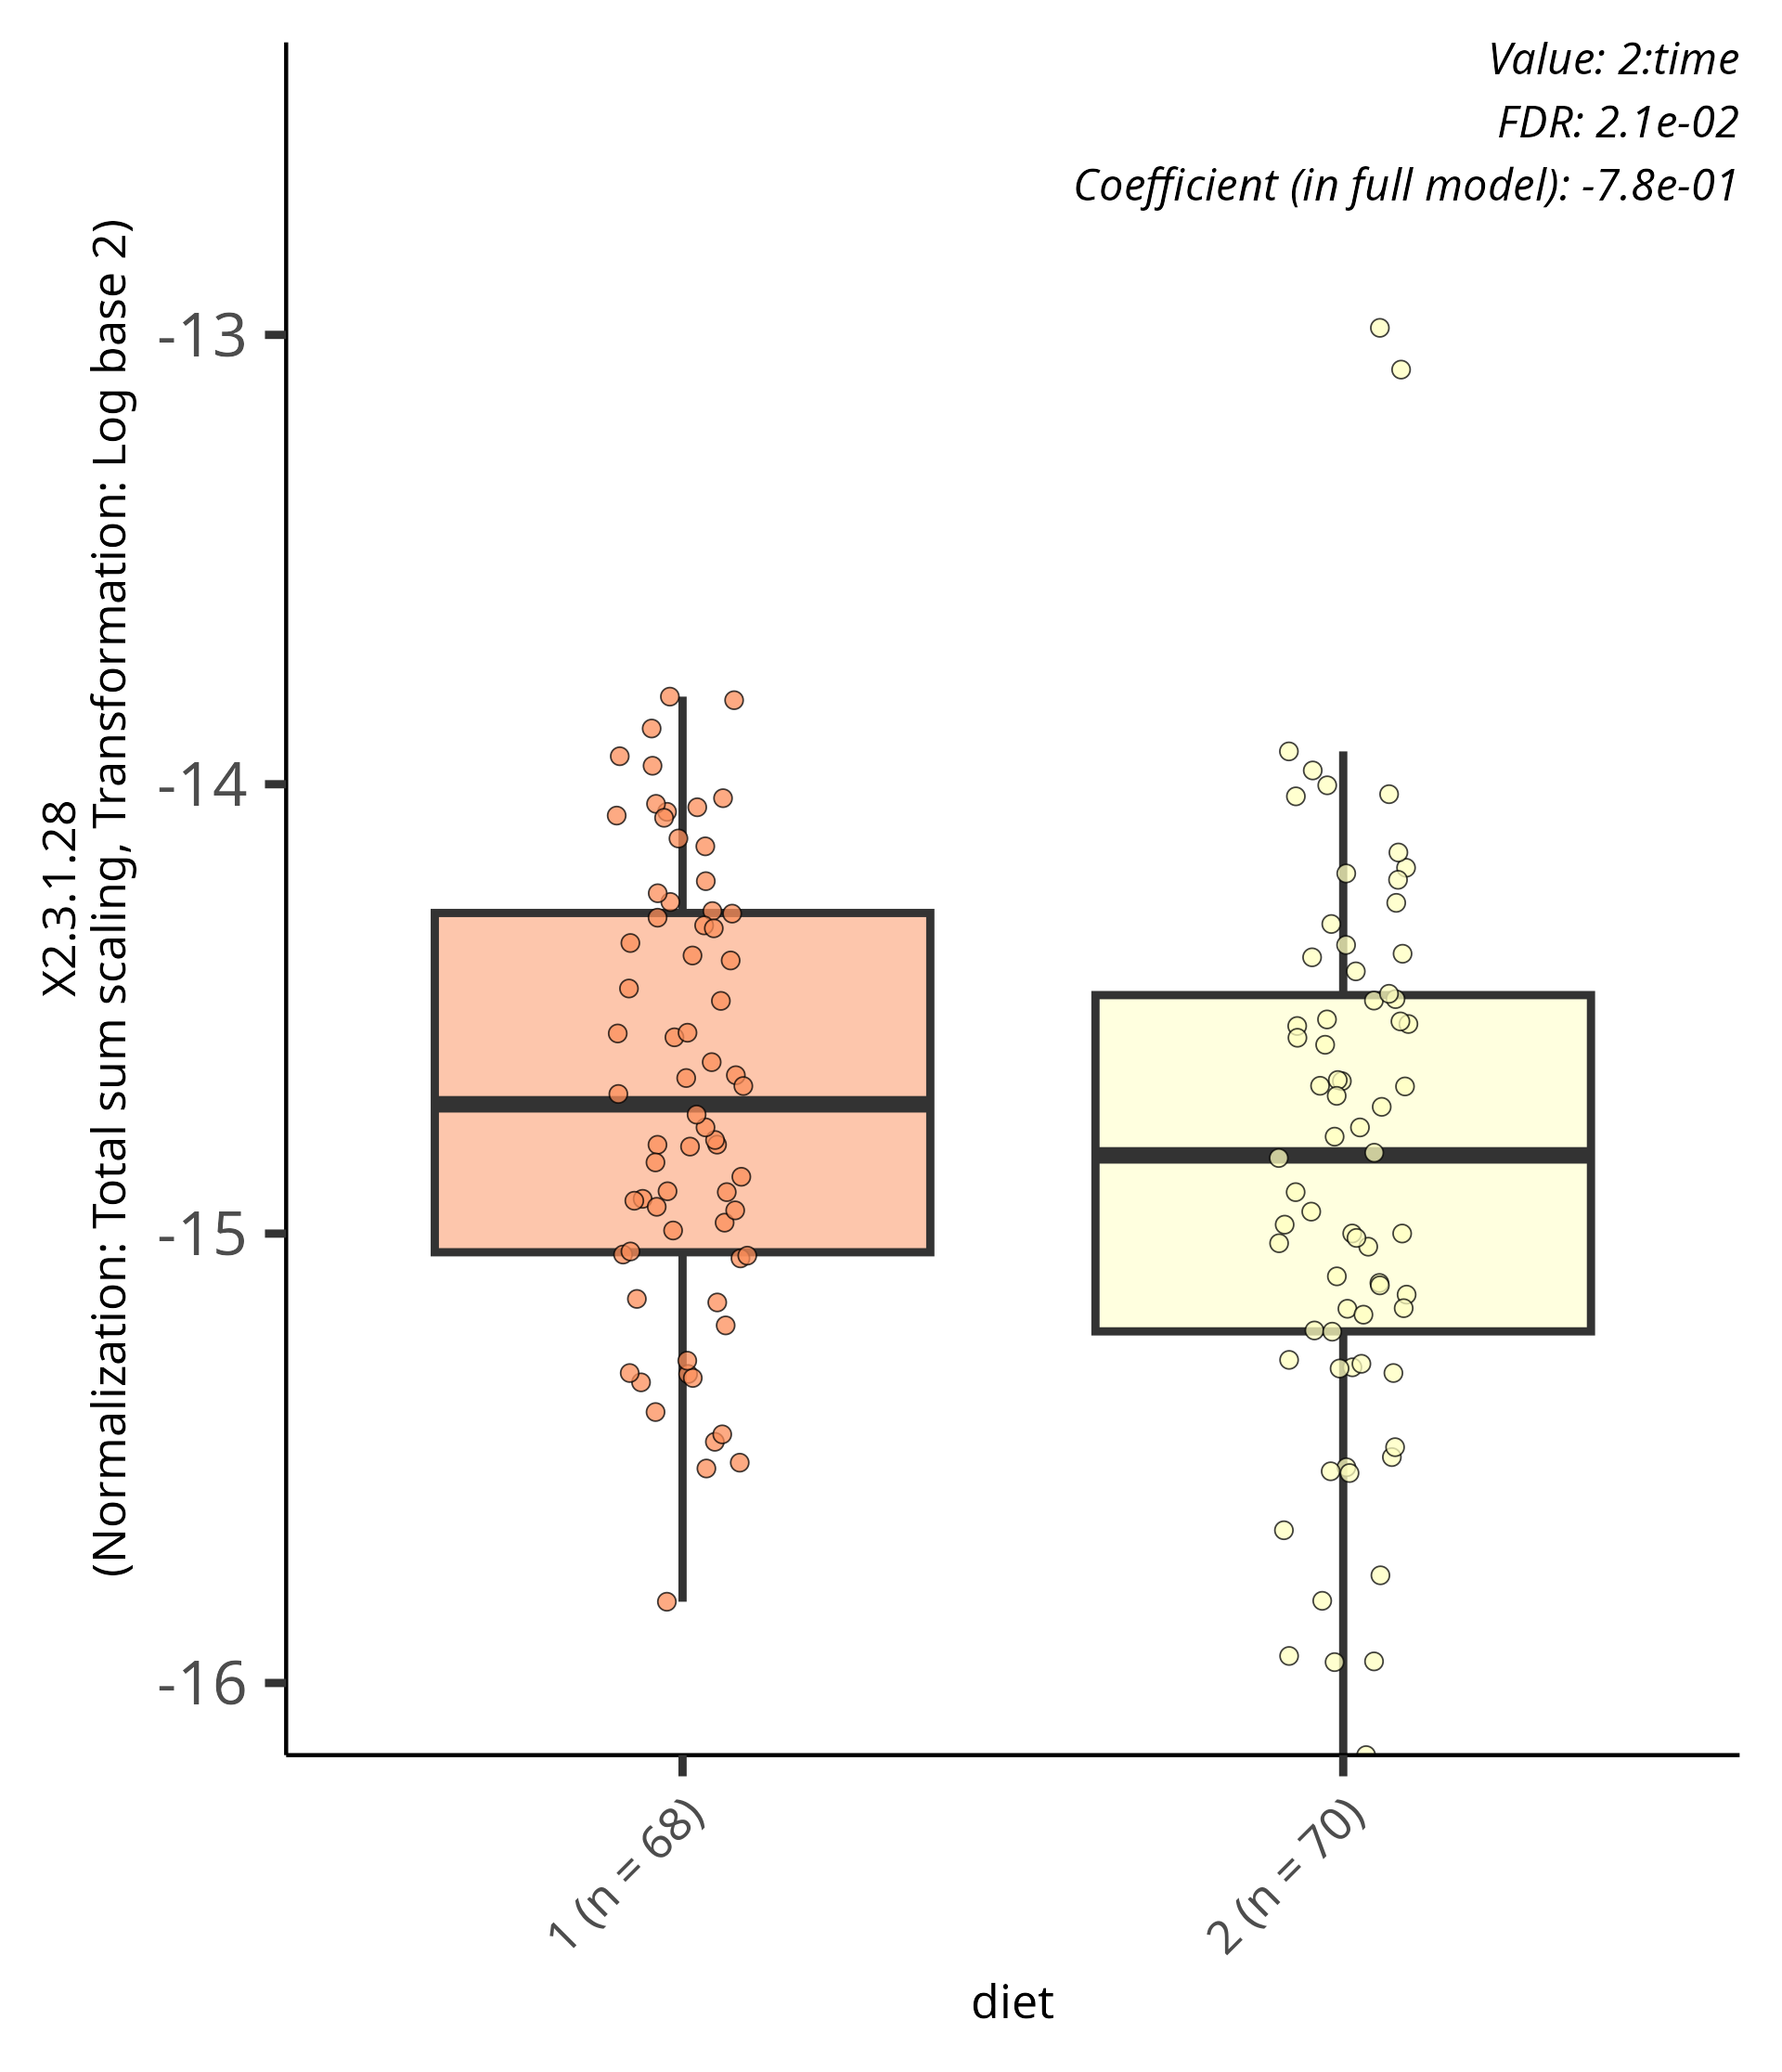
\includegraphics{../output/daa/daa_mtc/figures/association_plots/diet/linear/diet_X2.3.1.28_linear.png}\\
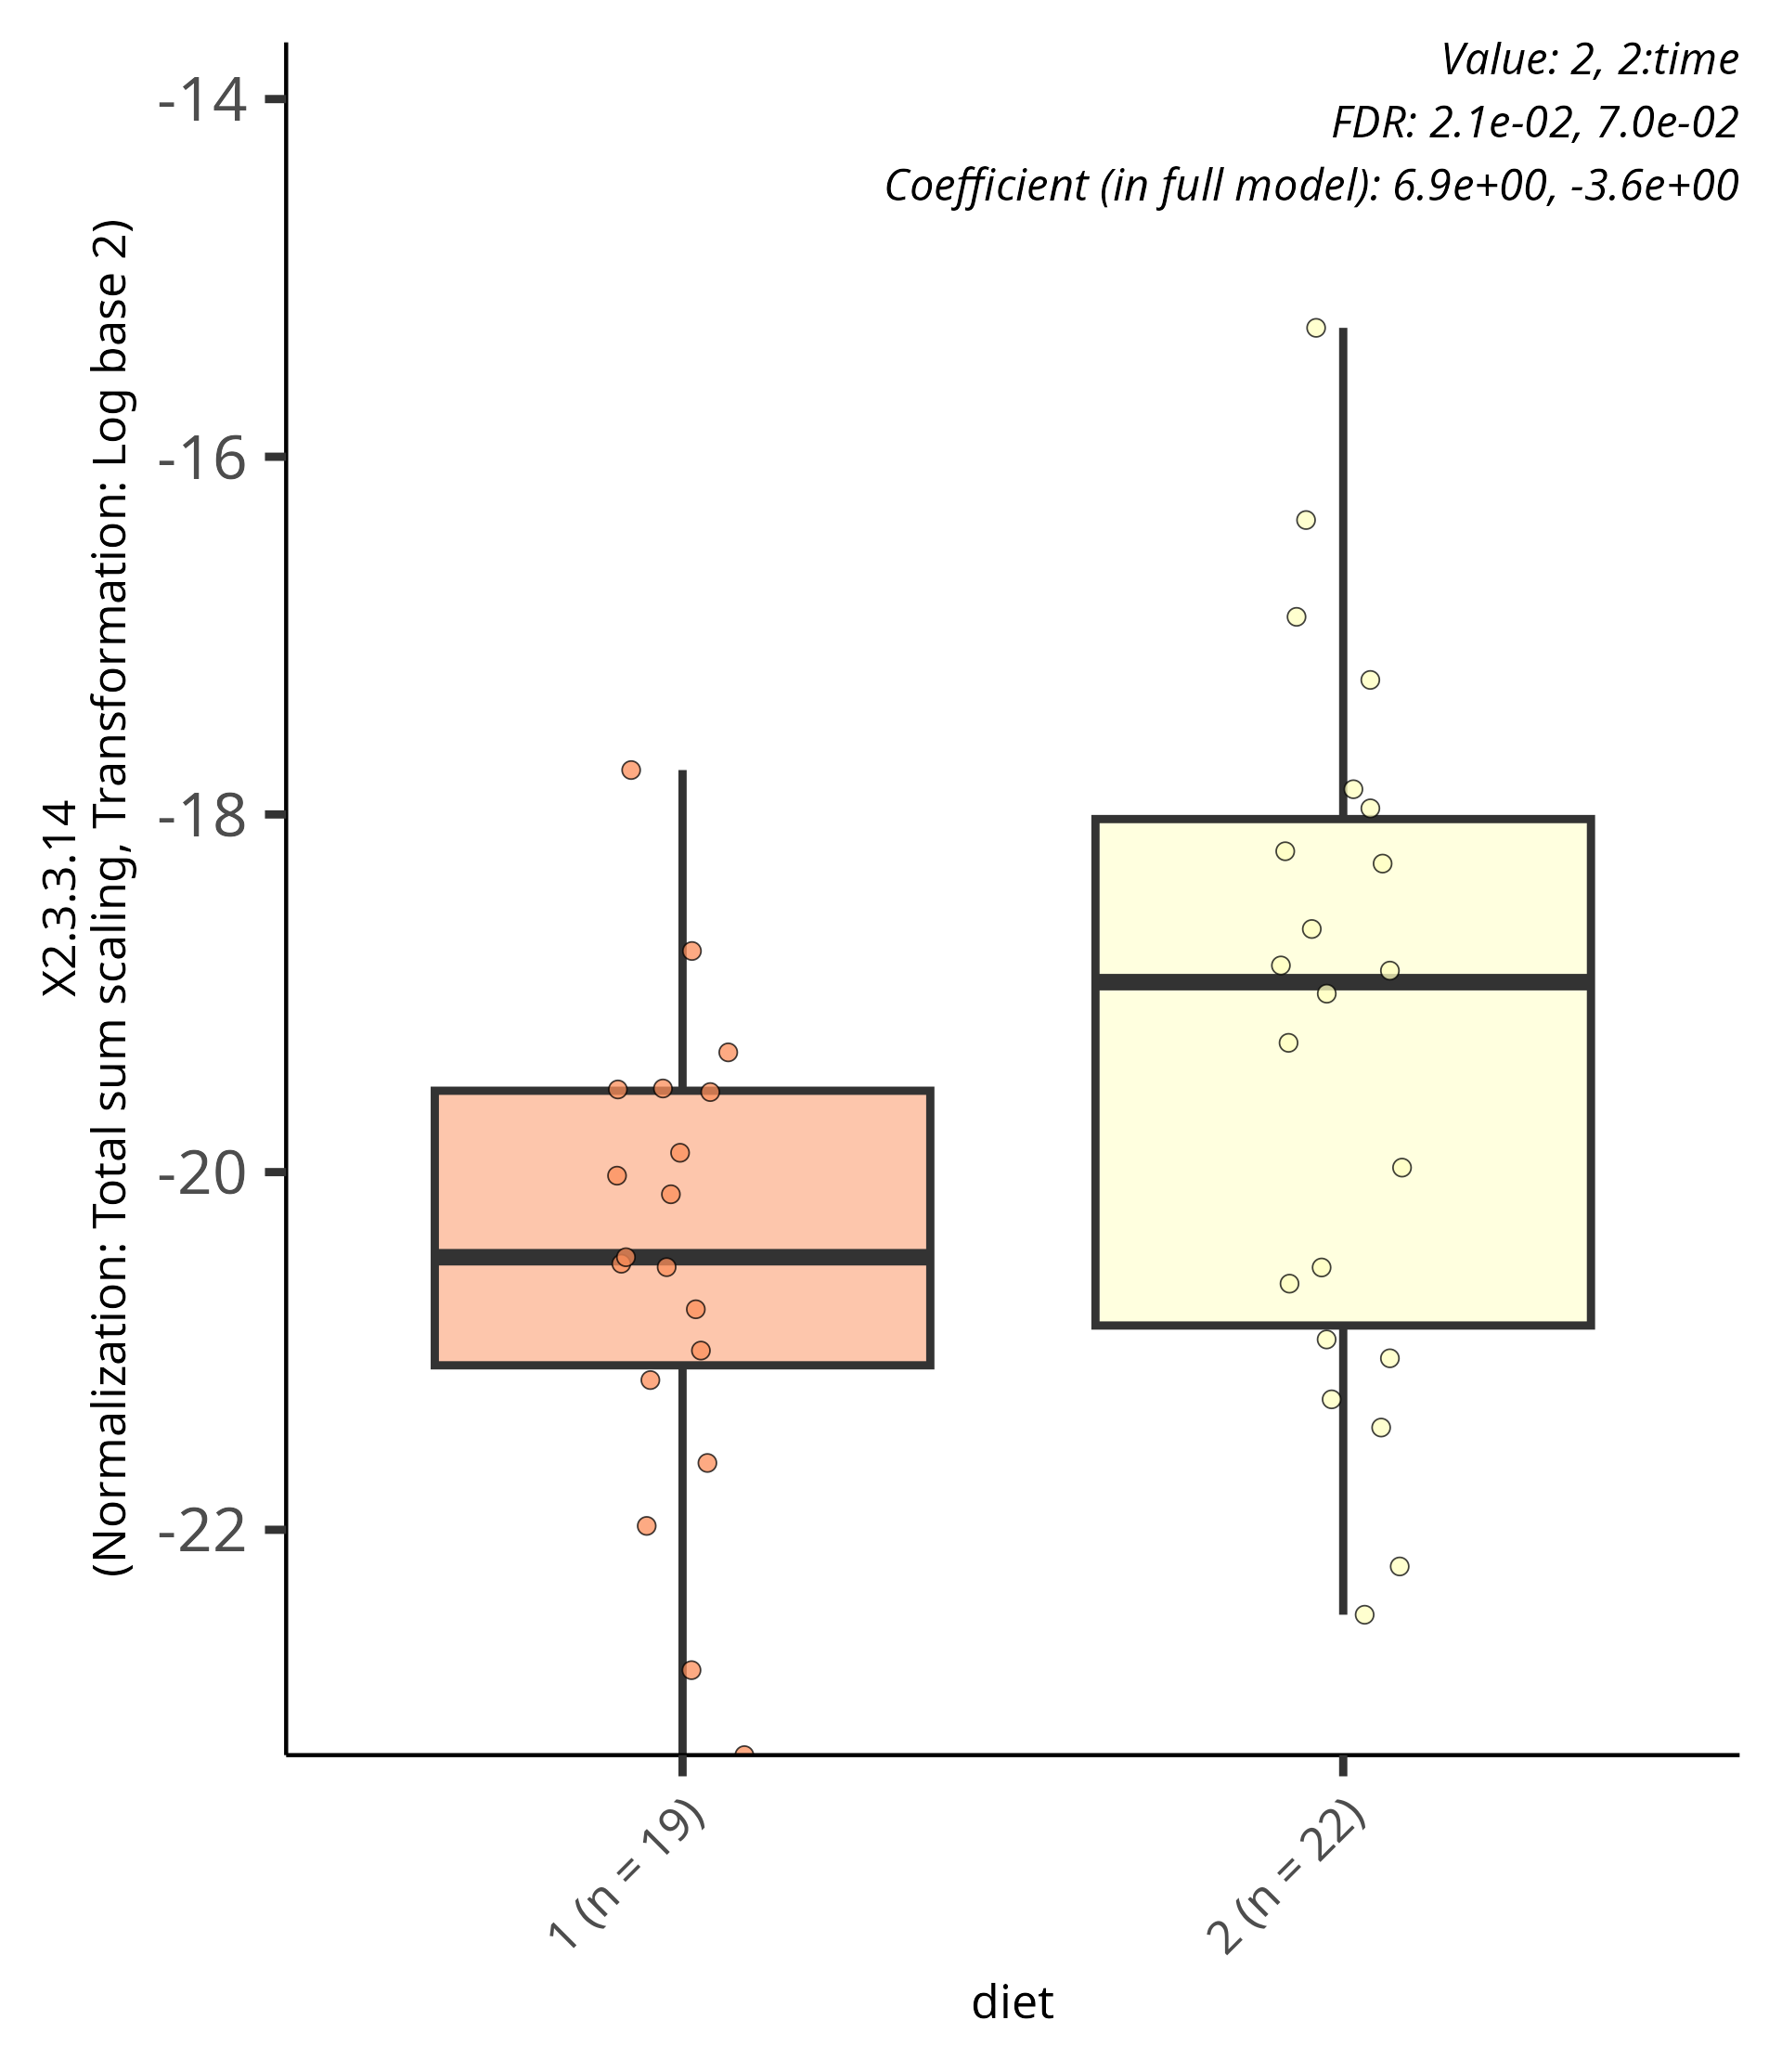
\includegraphics{../output/daa/daa_mtc/figures/association_plots/diet/linear/diet_X2.3.3.14_linear.png}\\
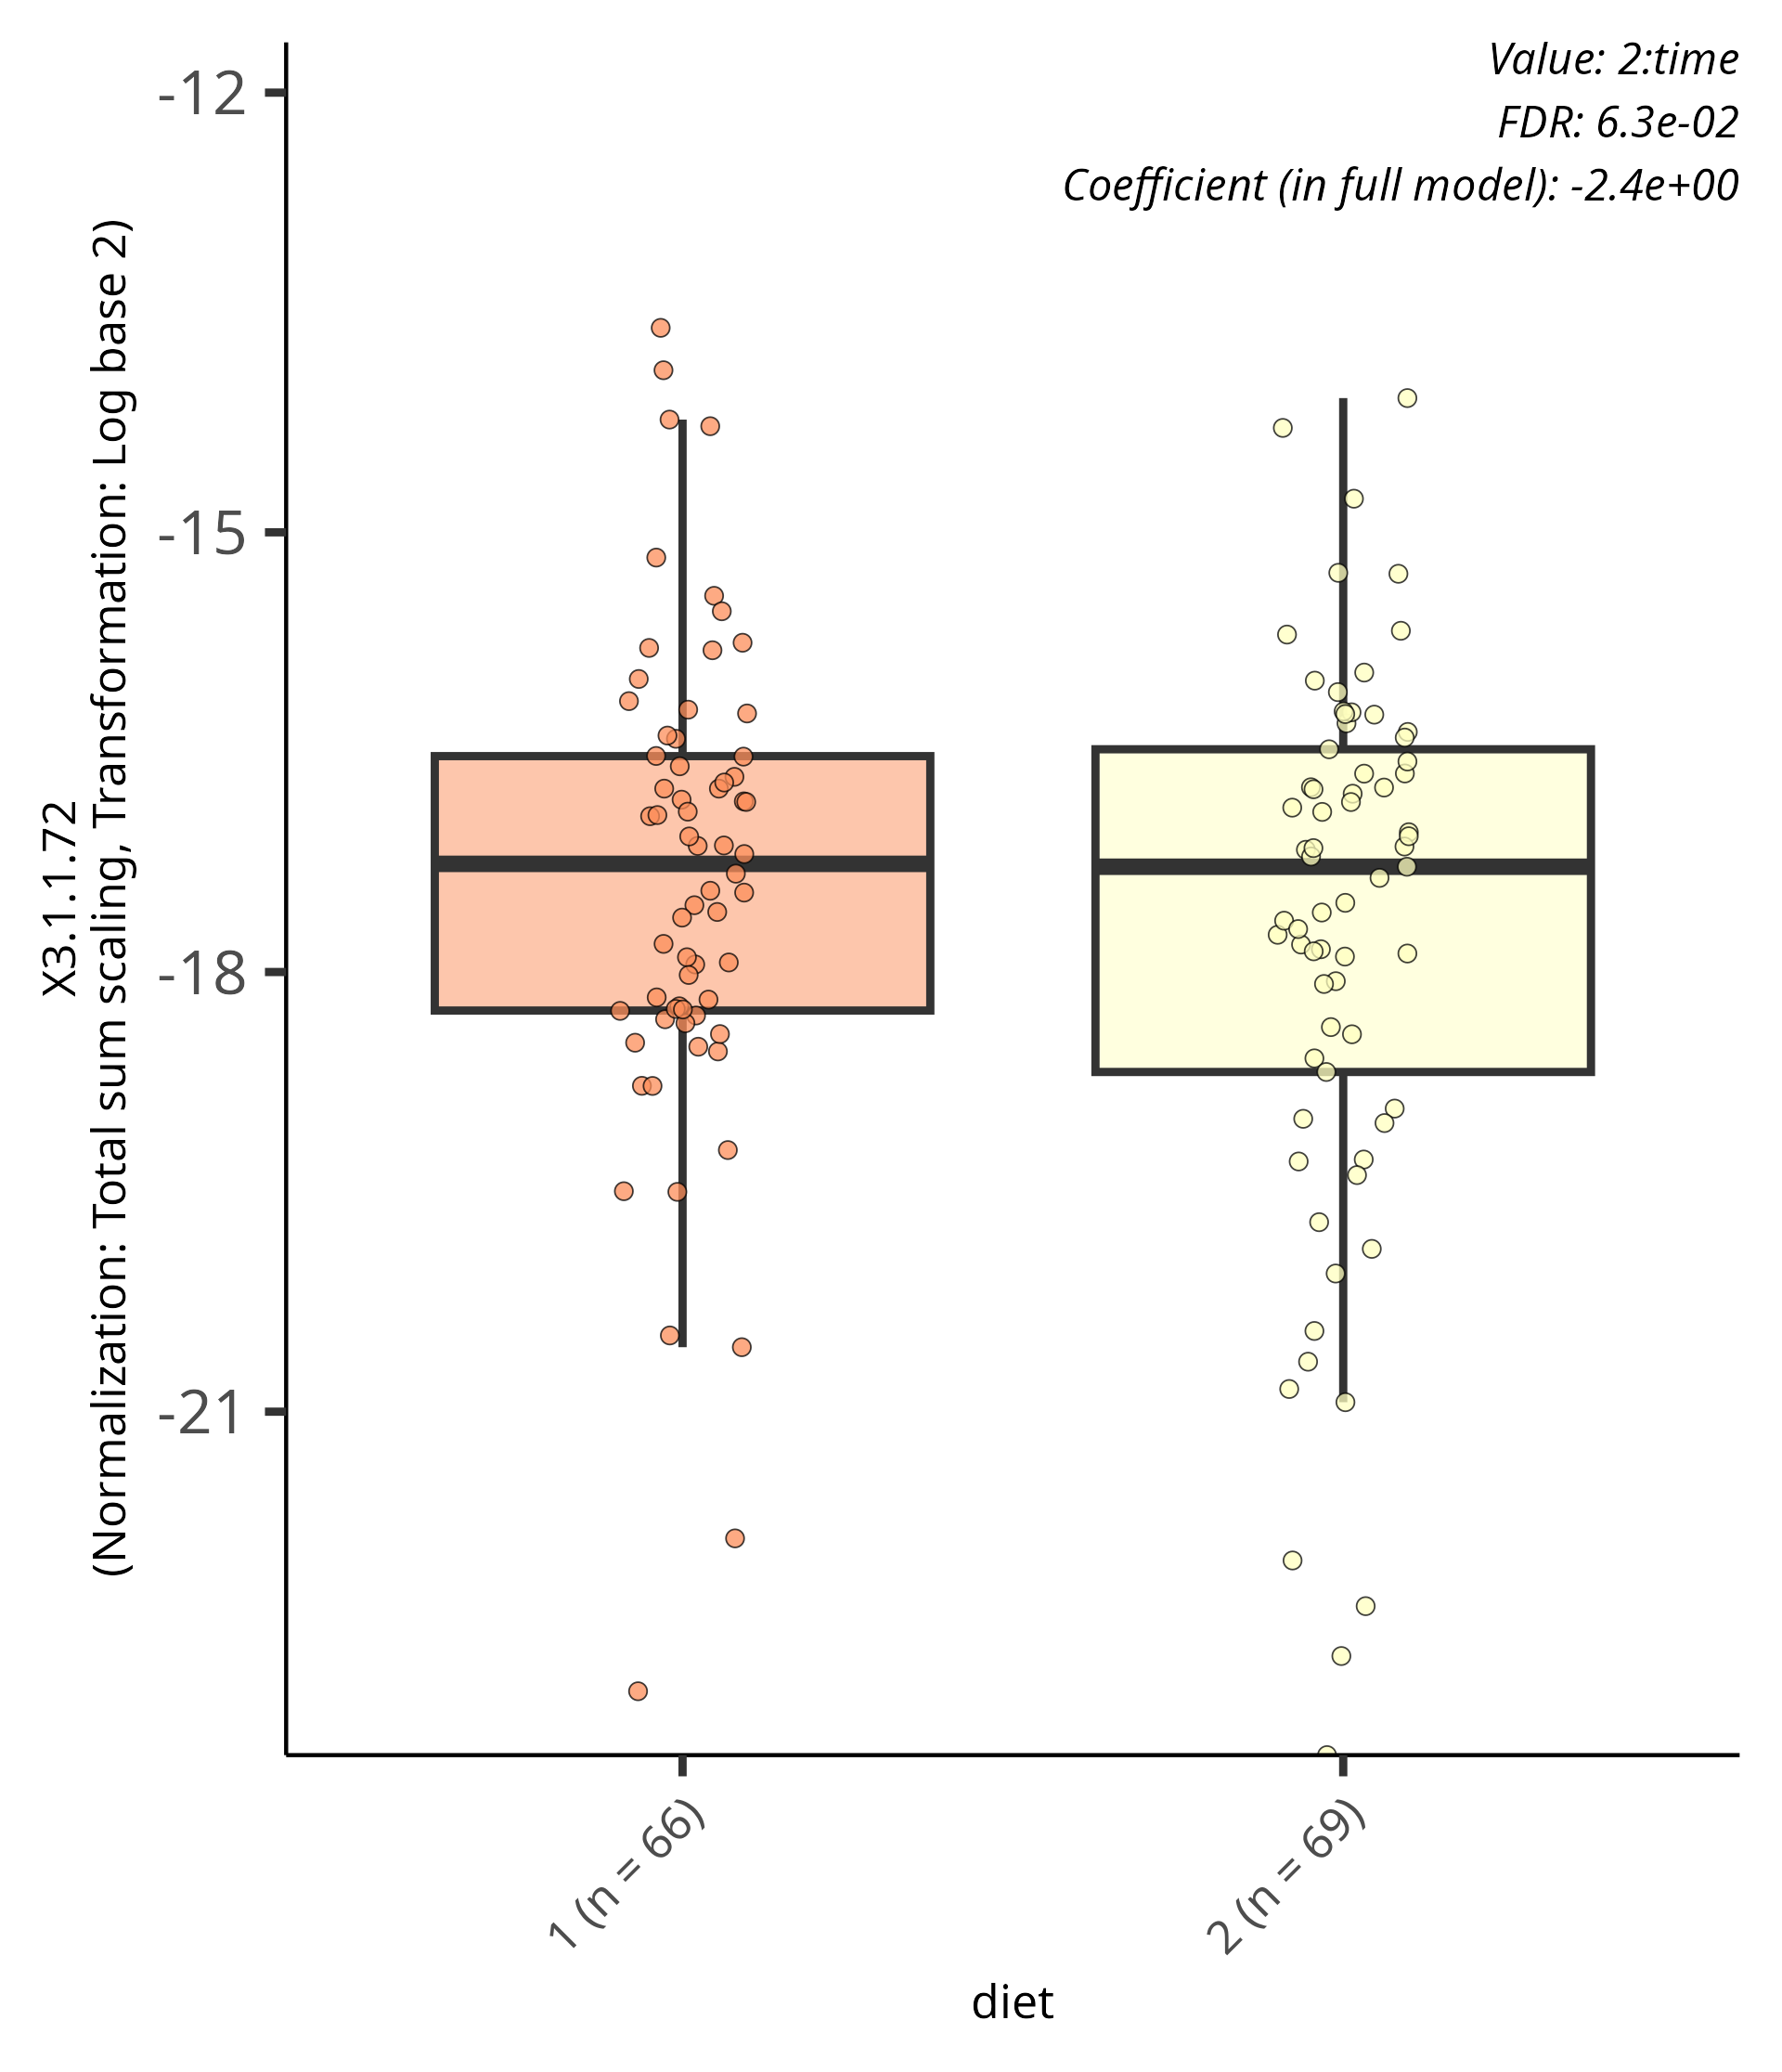
\includegraphics{../output/daa/daa_mtc/figures/association_plots/diet/linear/diet_X3.1.1.72_linear.png}\\
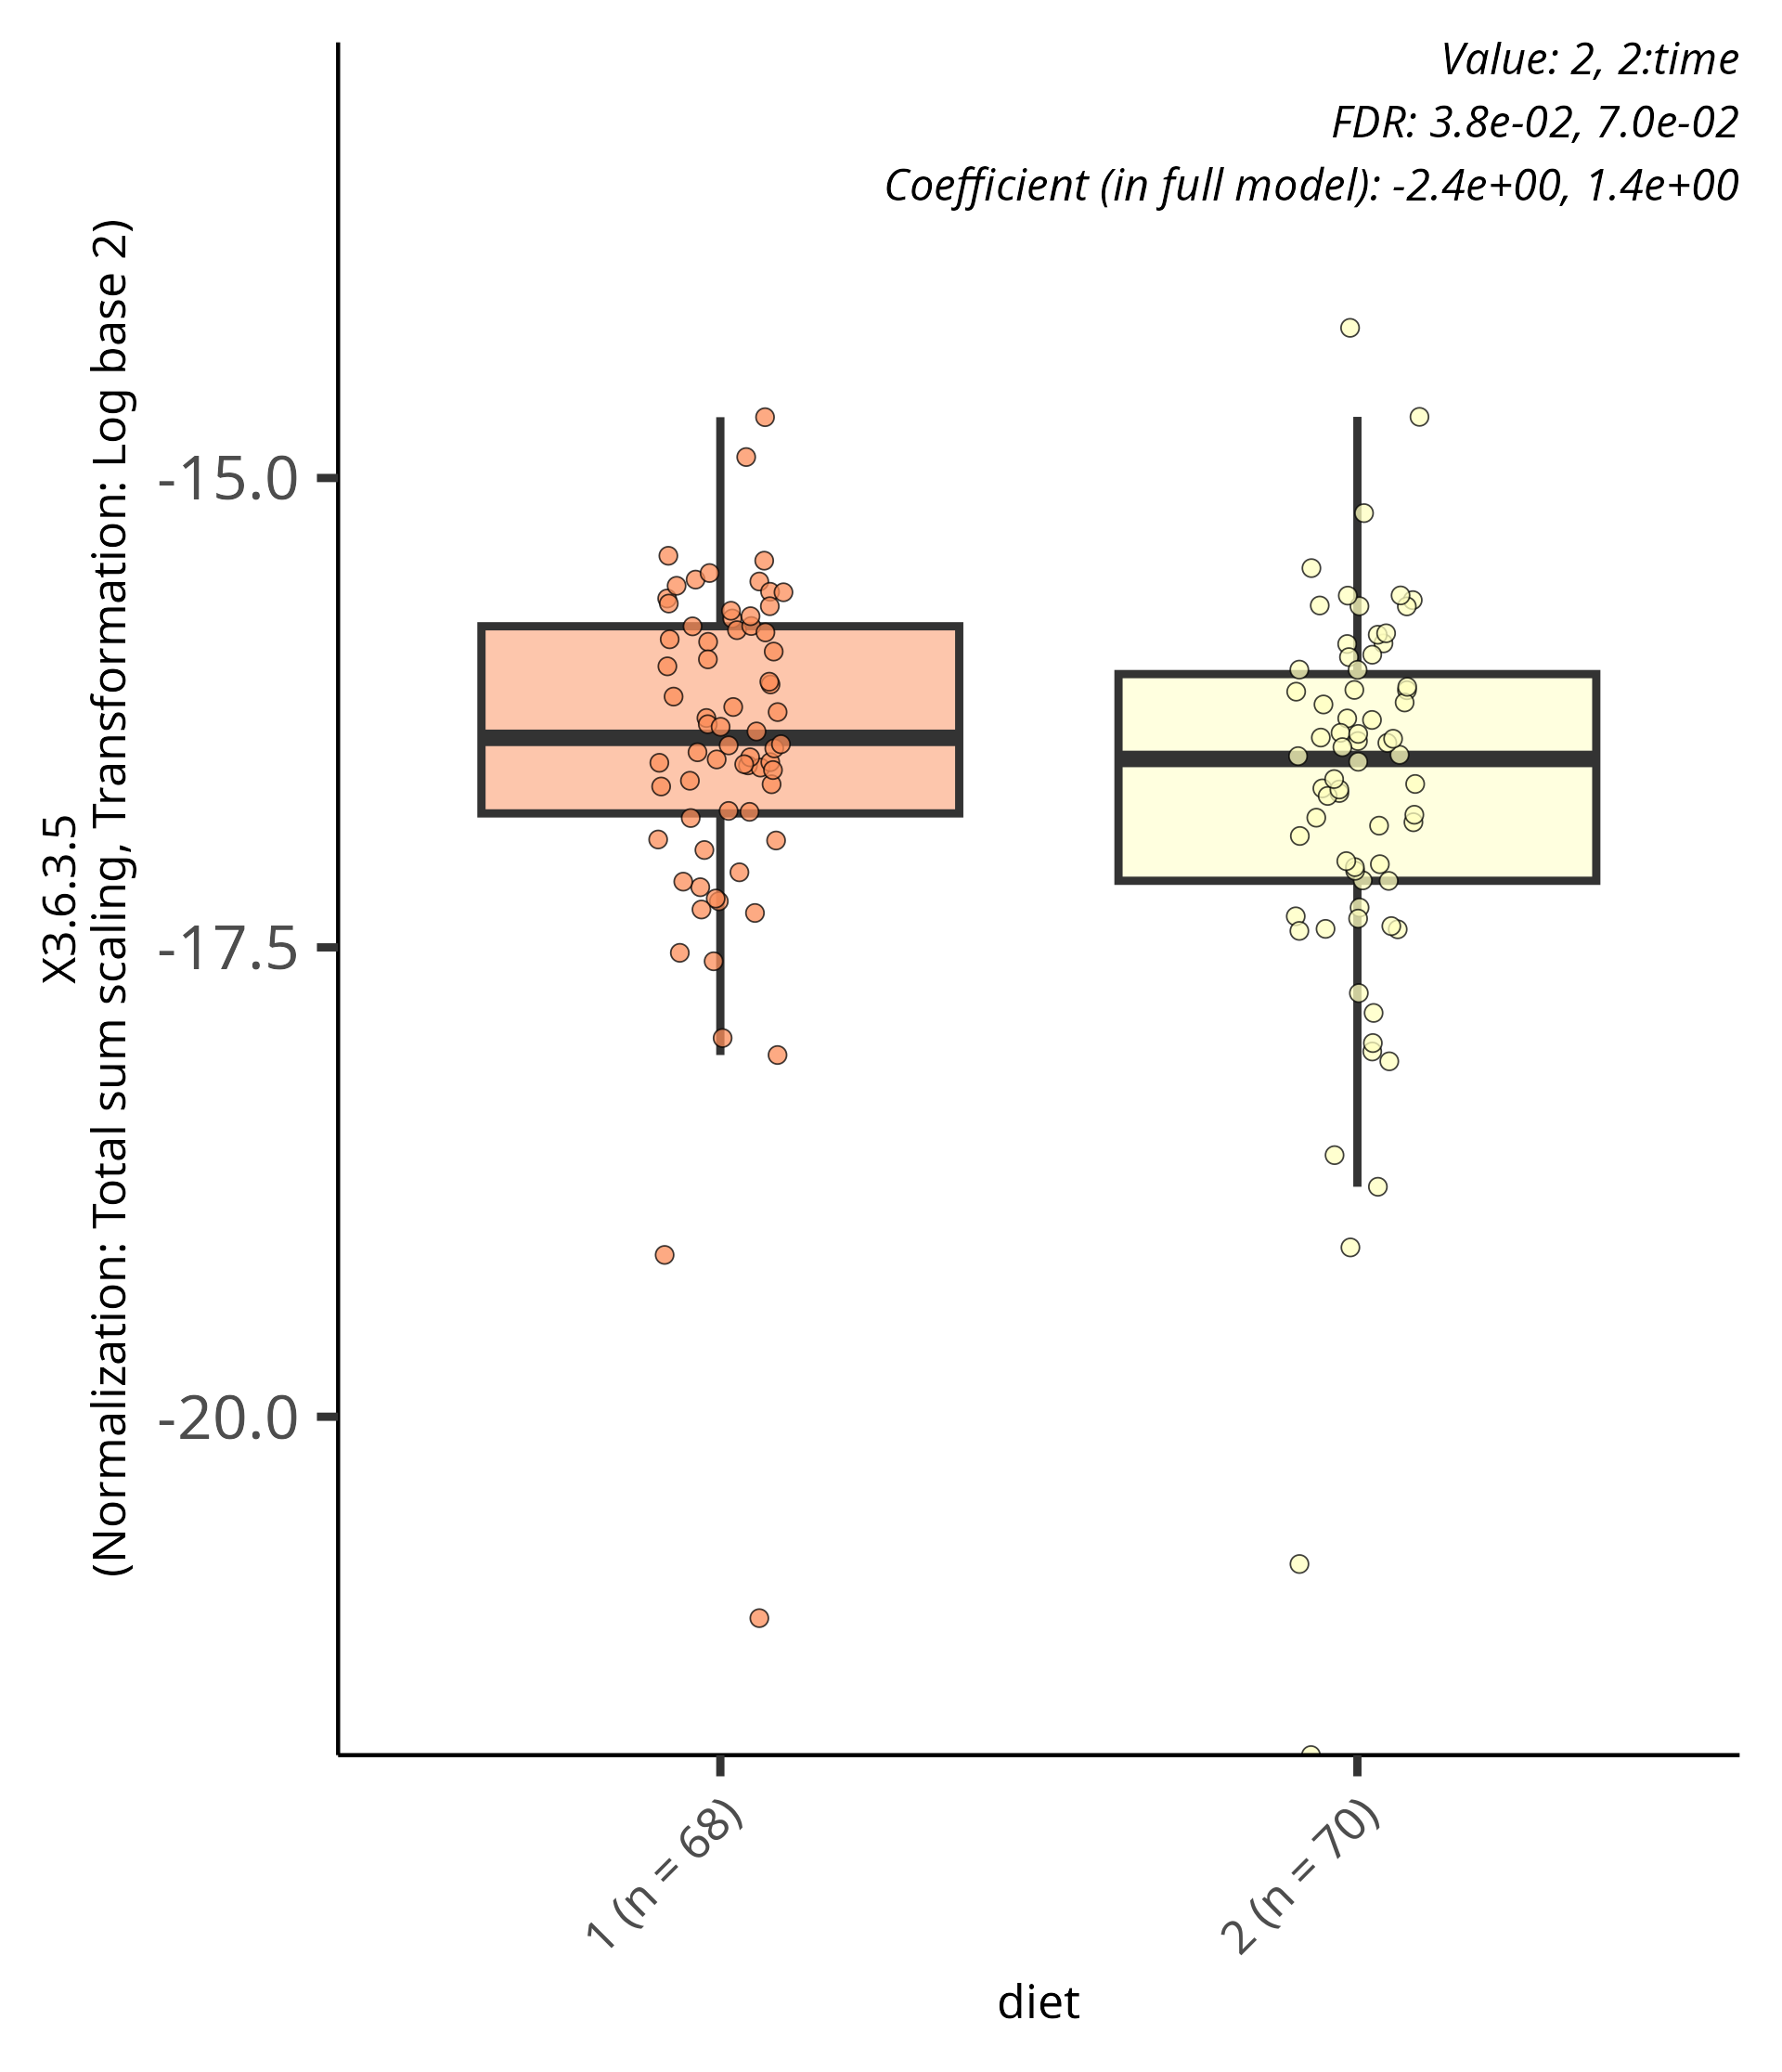
\includegraphics{../output/daa/daa_mtc/figures/association_plots/diet/linear/diet_X3.6.3.5_linear.png}\\
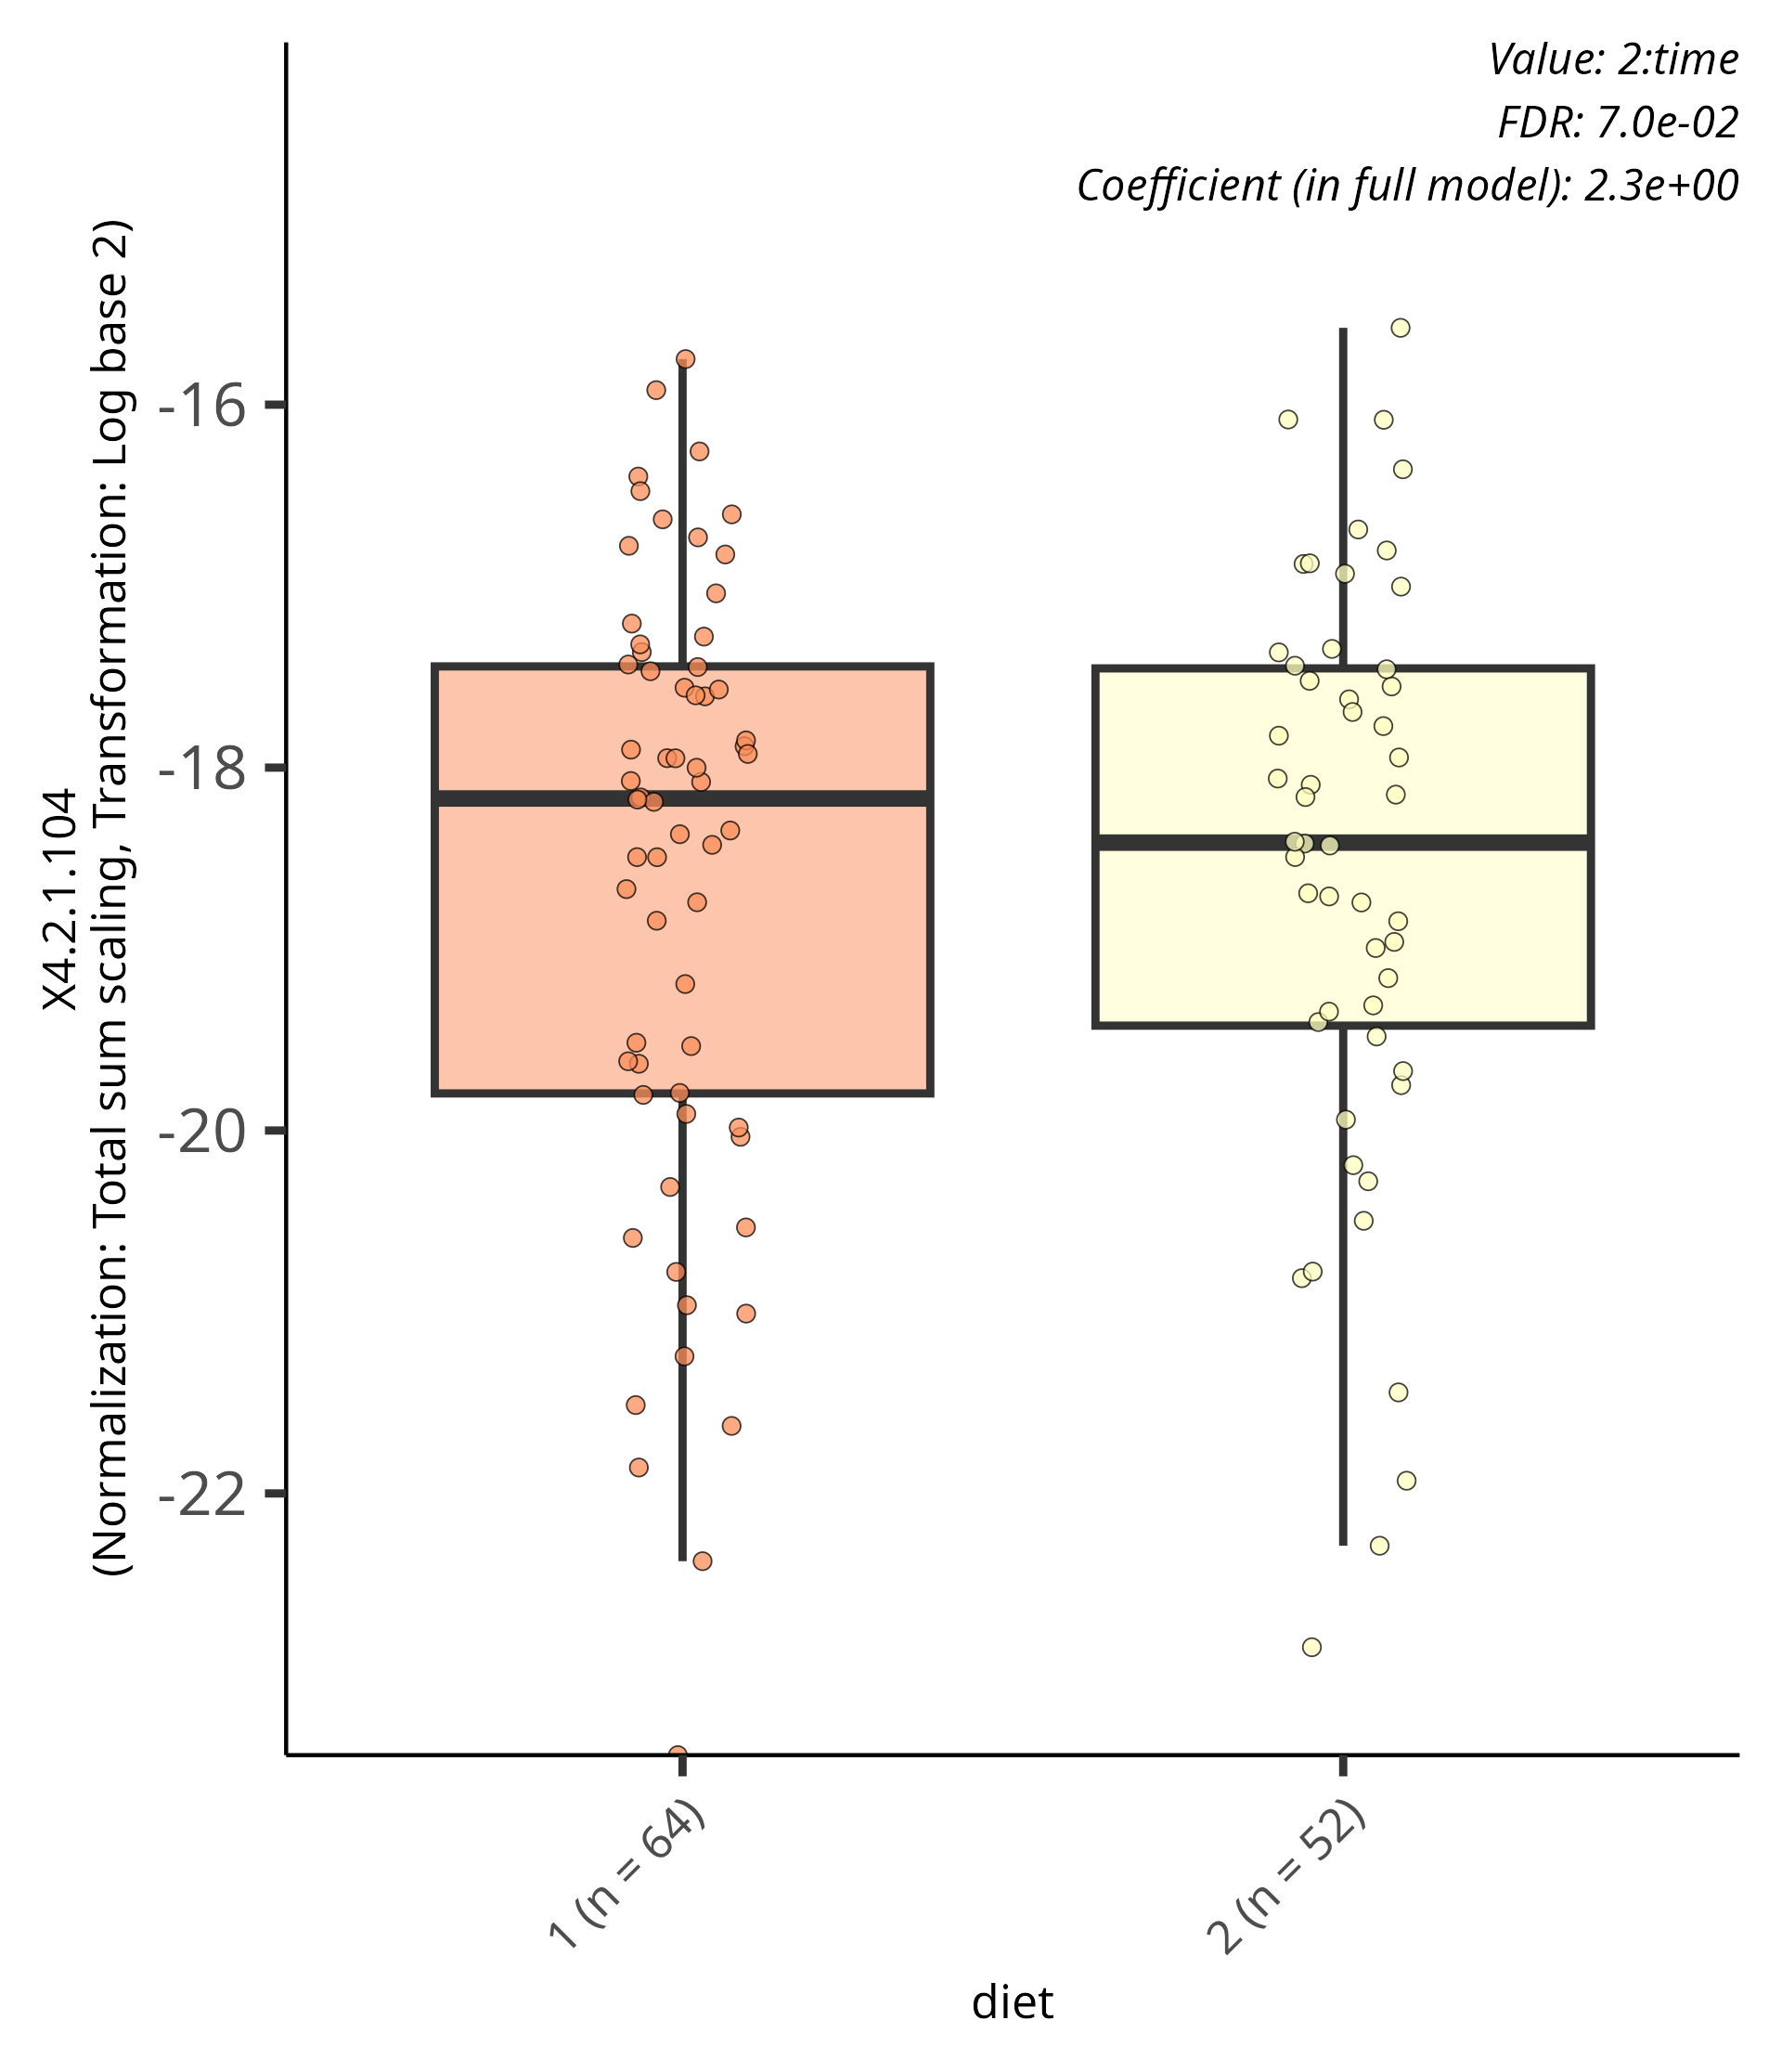
\includegraphics{../output/daa/daa_mtc/figures/association_plots/diet/linear/diet_X4.2.1.104_linear.png}\\
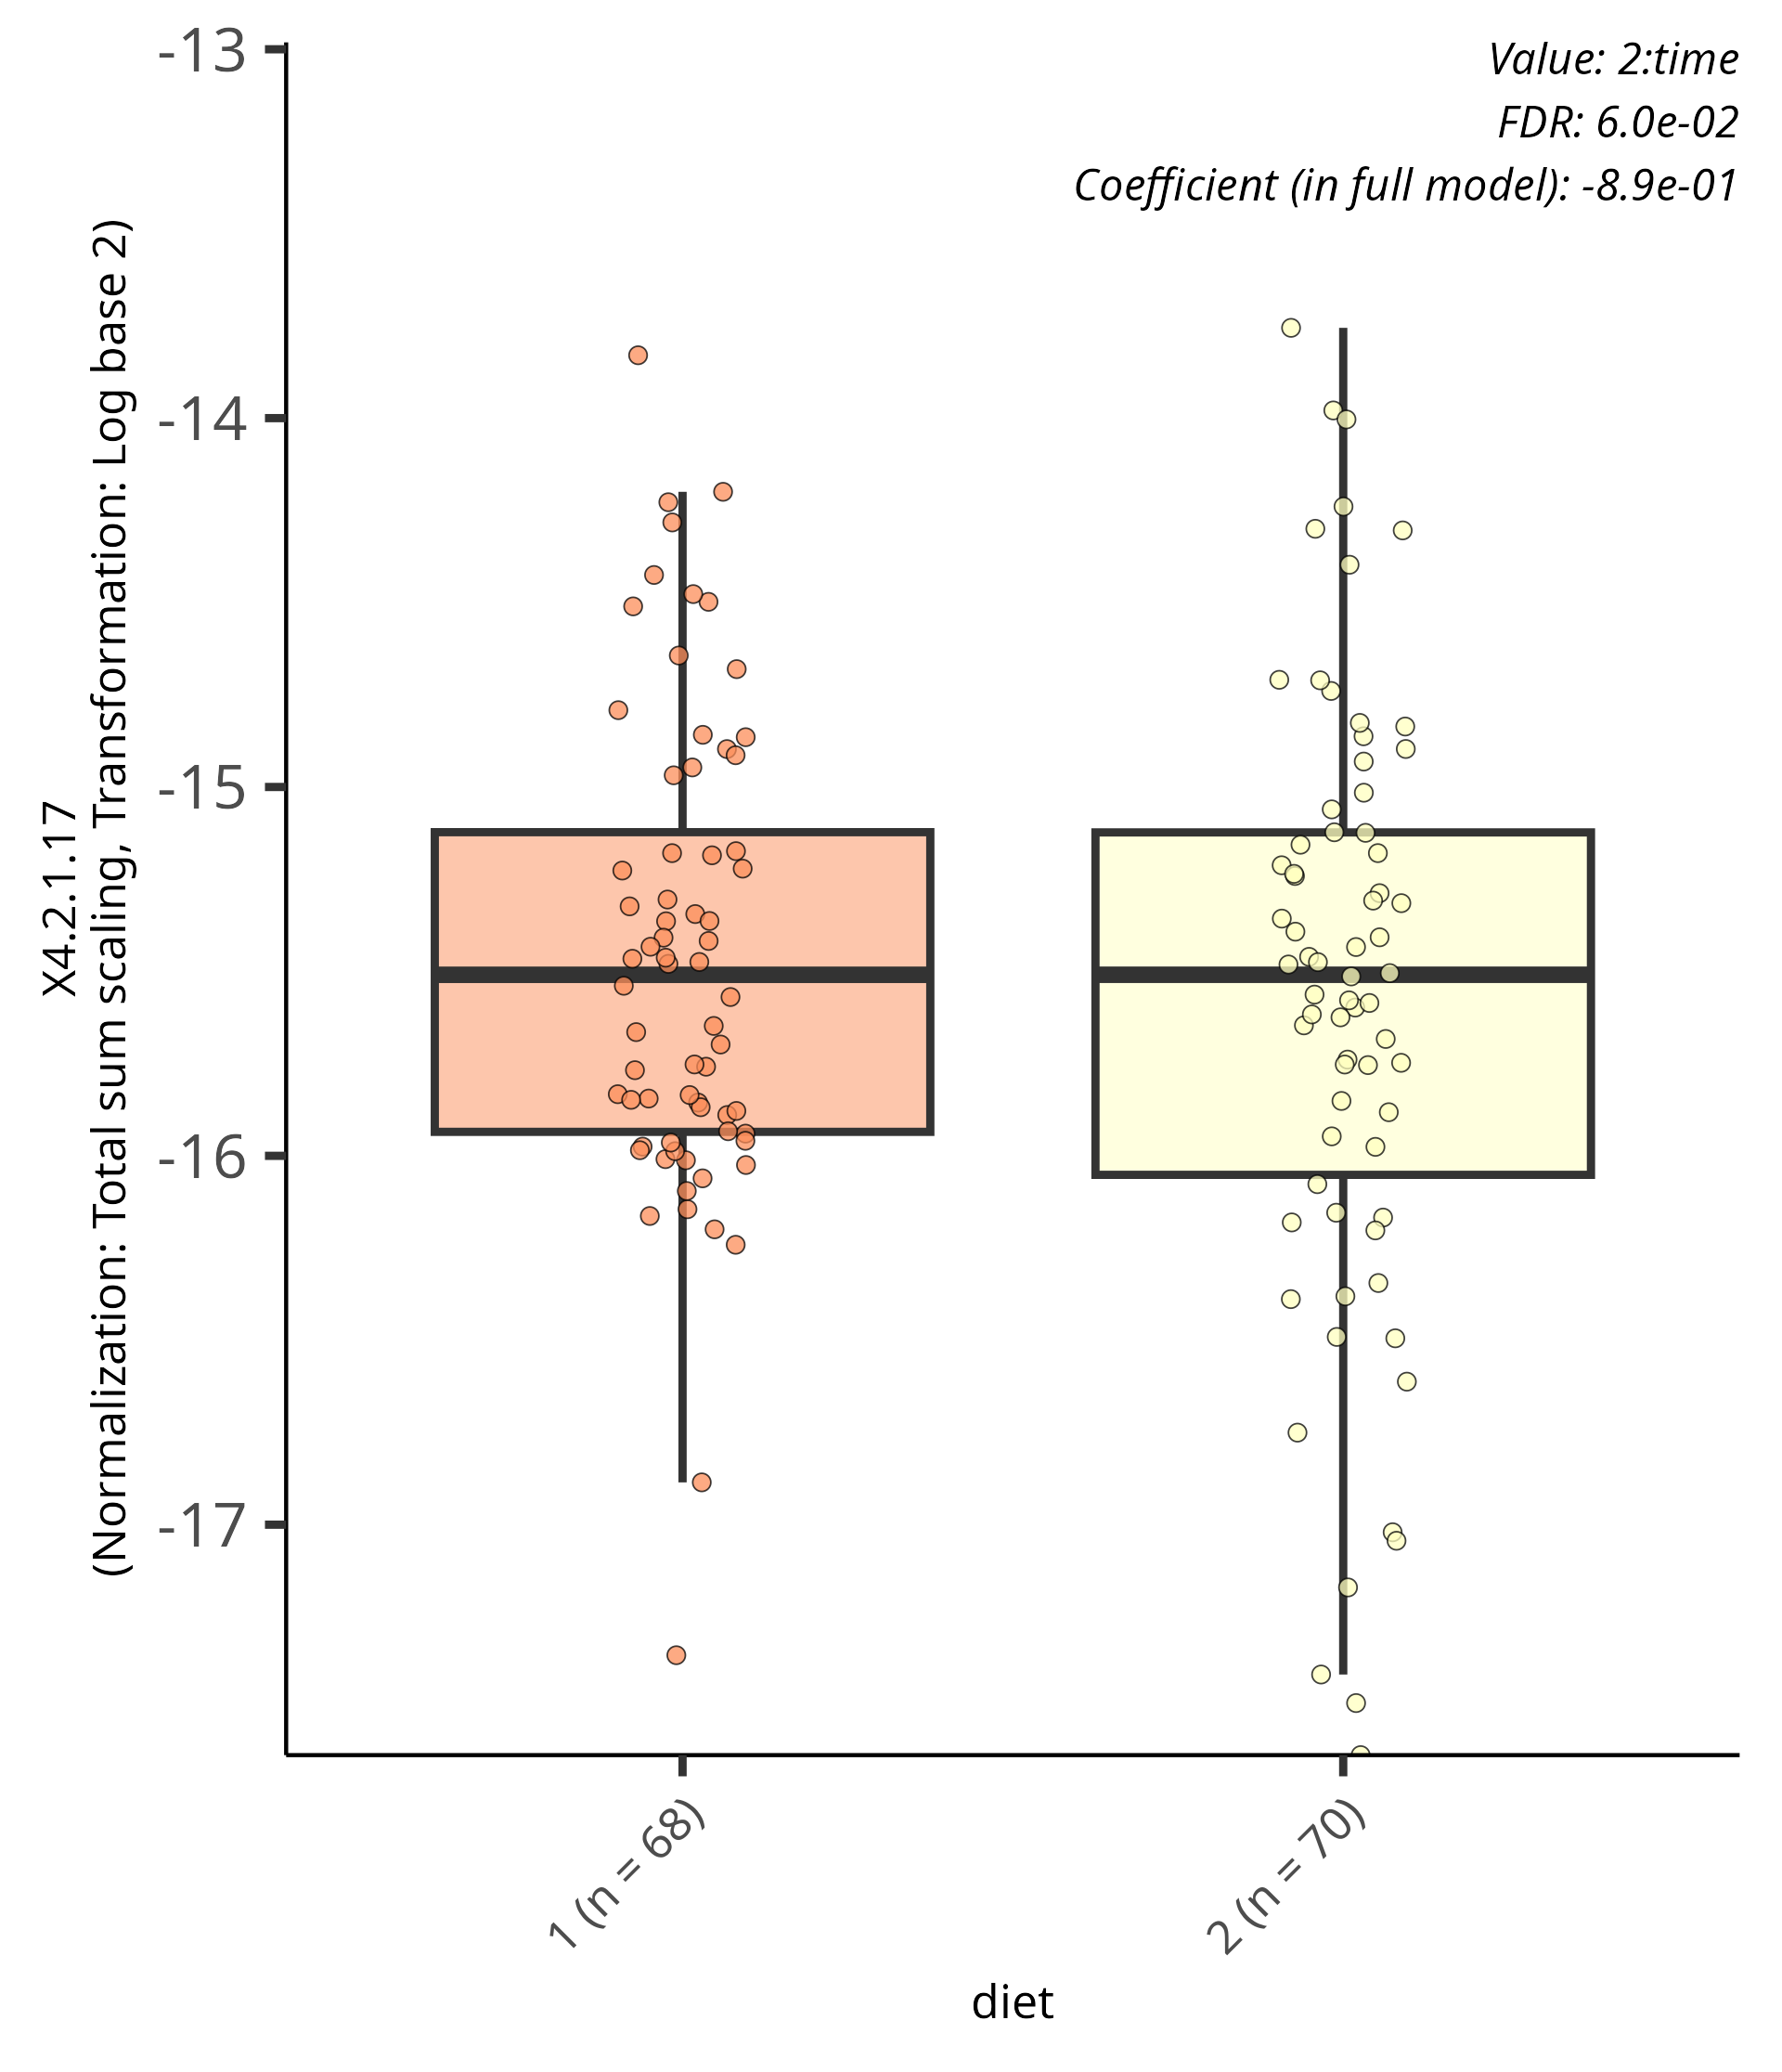
\includegraphics{../output/daa/daa_mtc/figures/association_plots/diet/linear/diet_X4.2.1.17_linear.png}\\
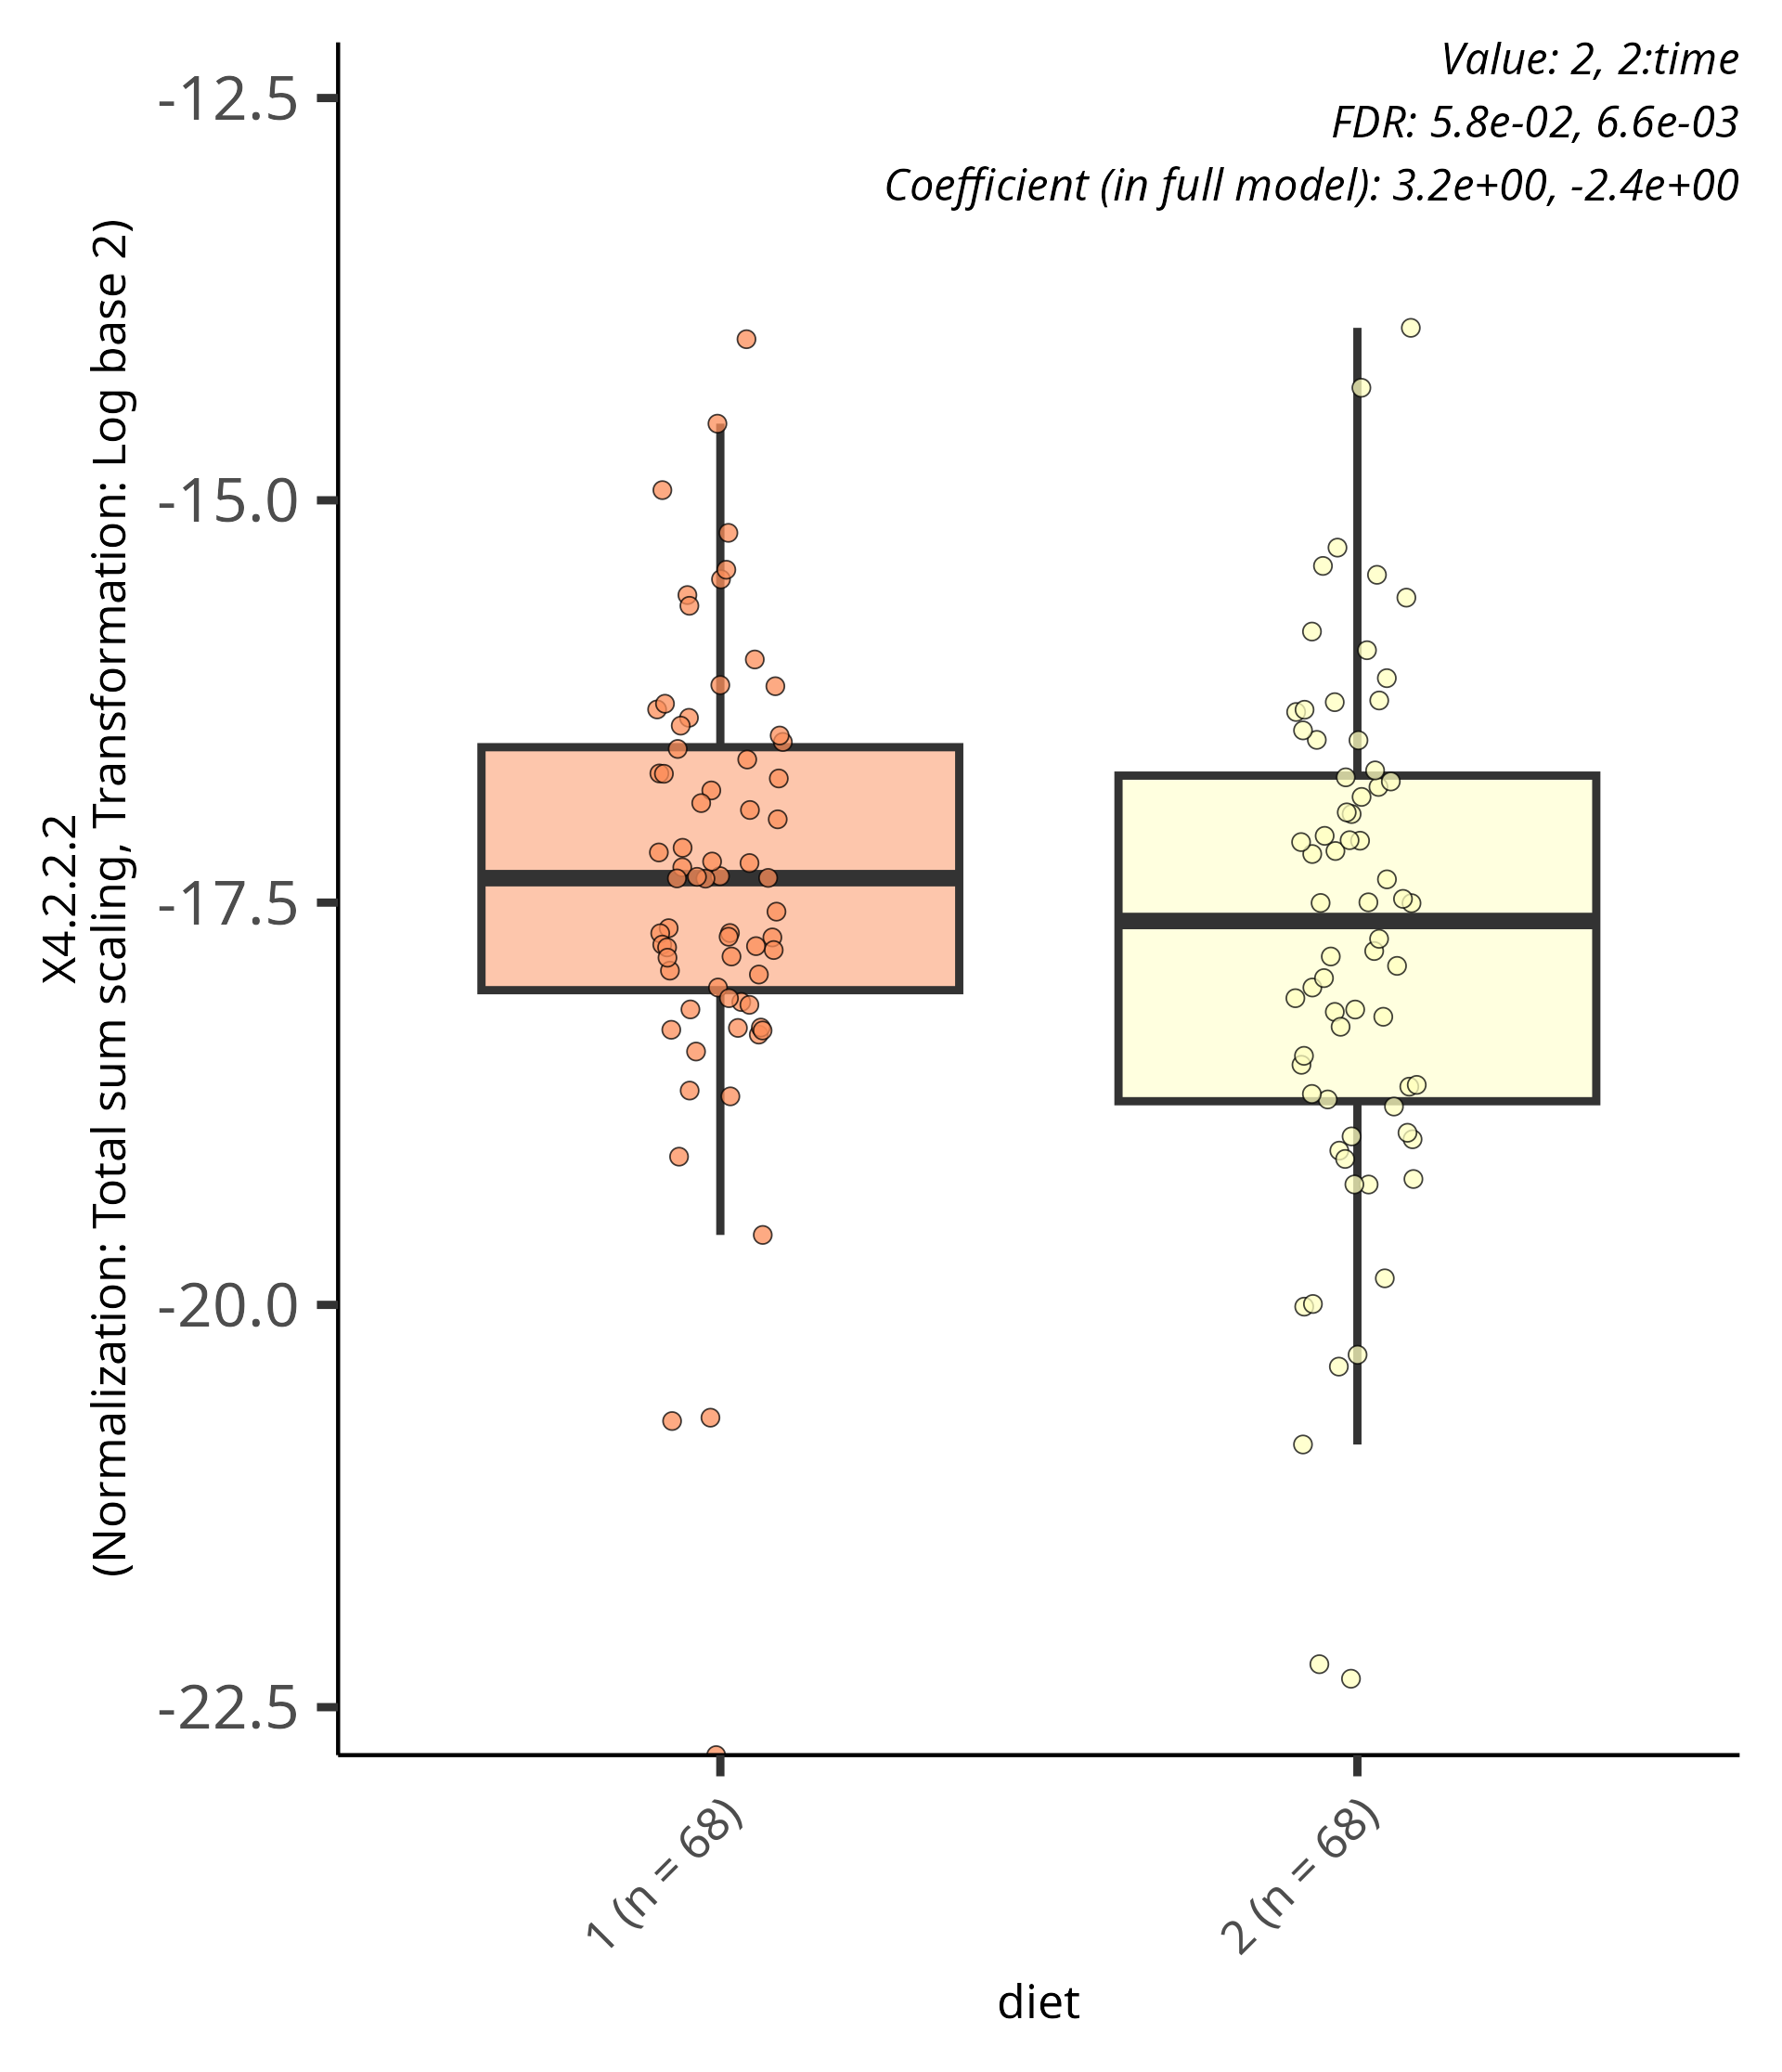
\includegraphics{../output/daa/daa_mtc/figures/association_plots/diet/linear/diet_X4.2.2.2_linear.png}\\
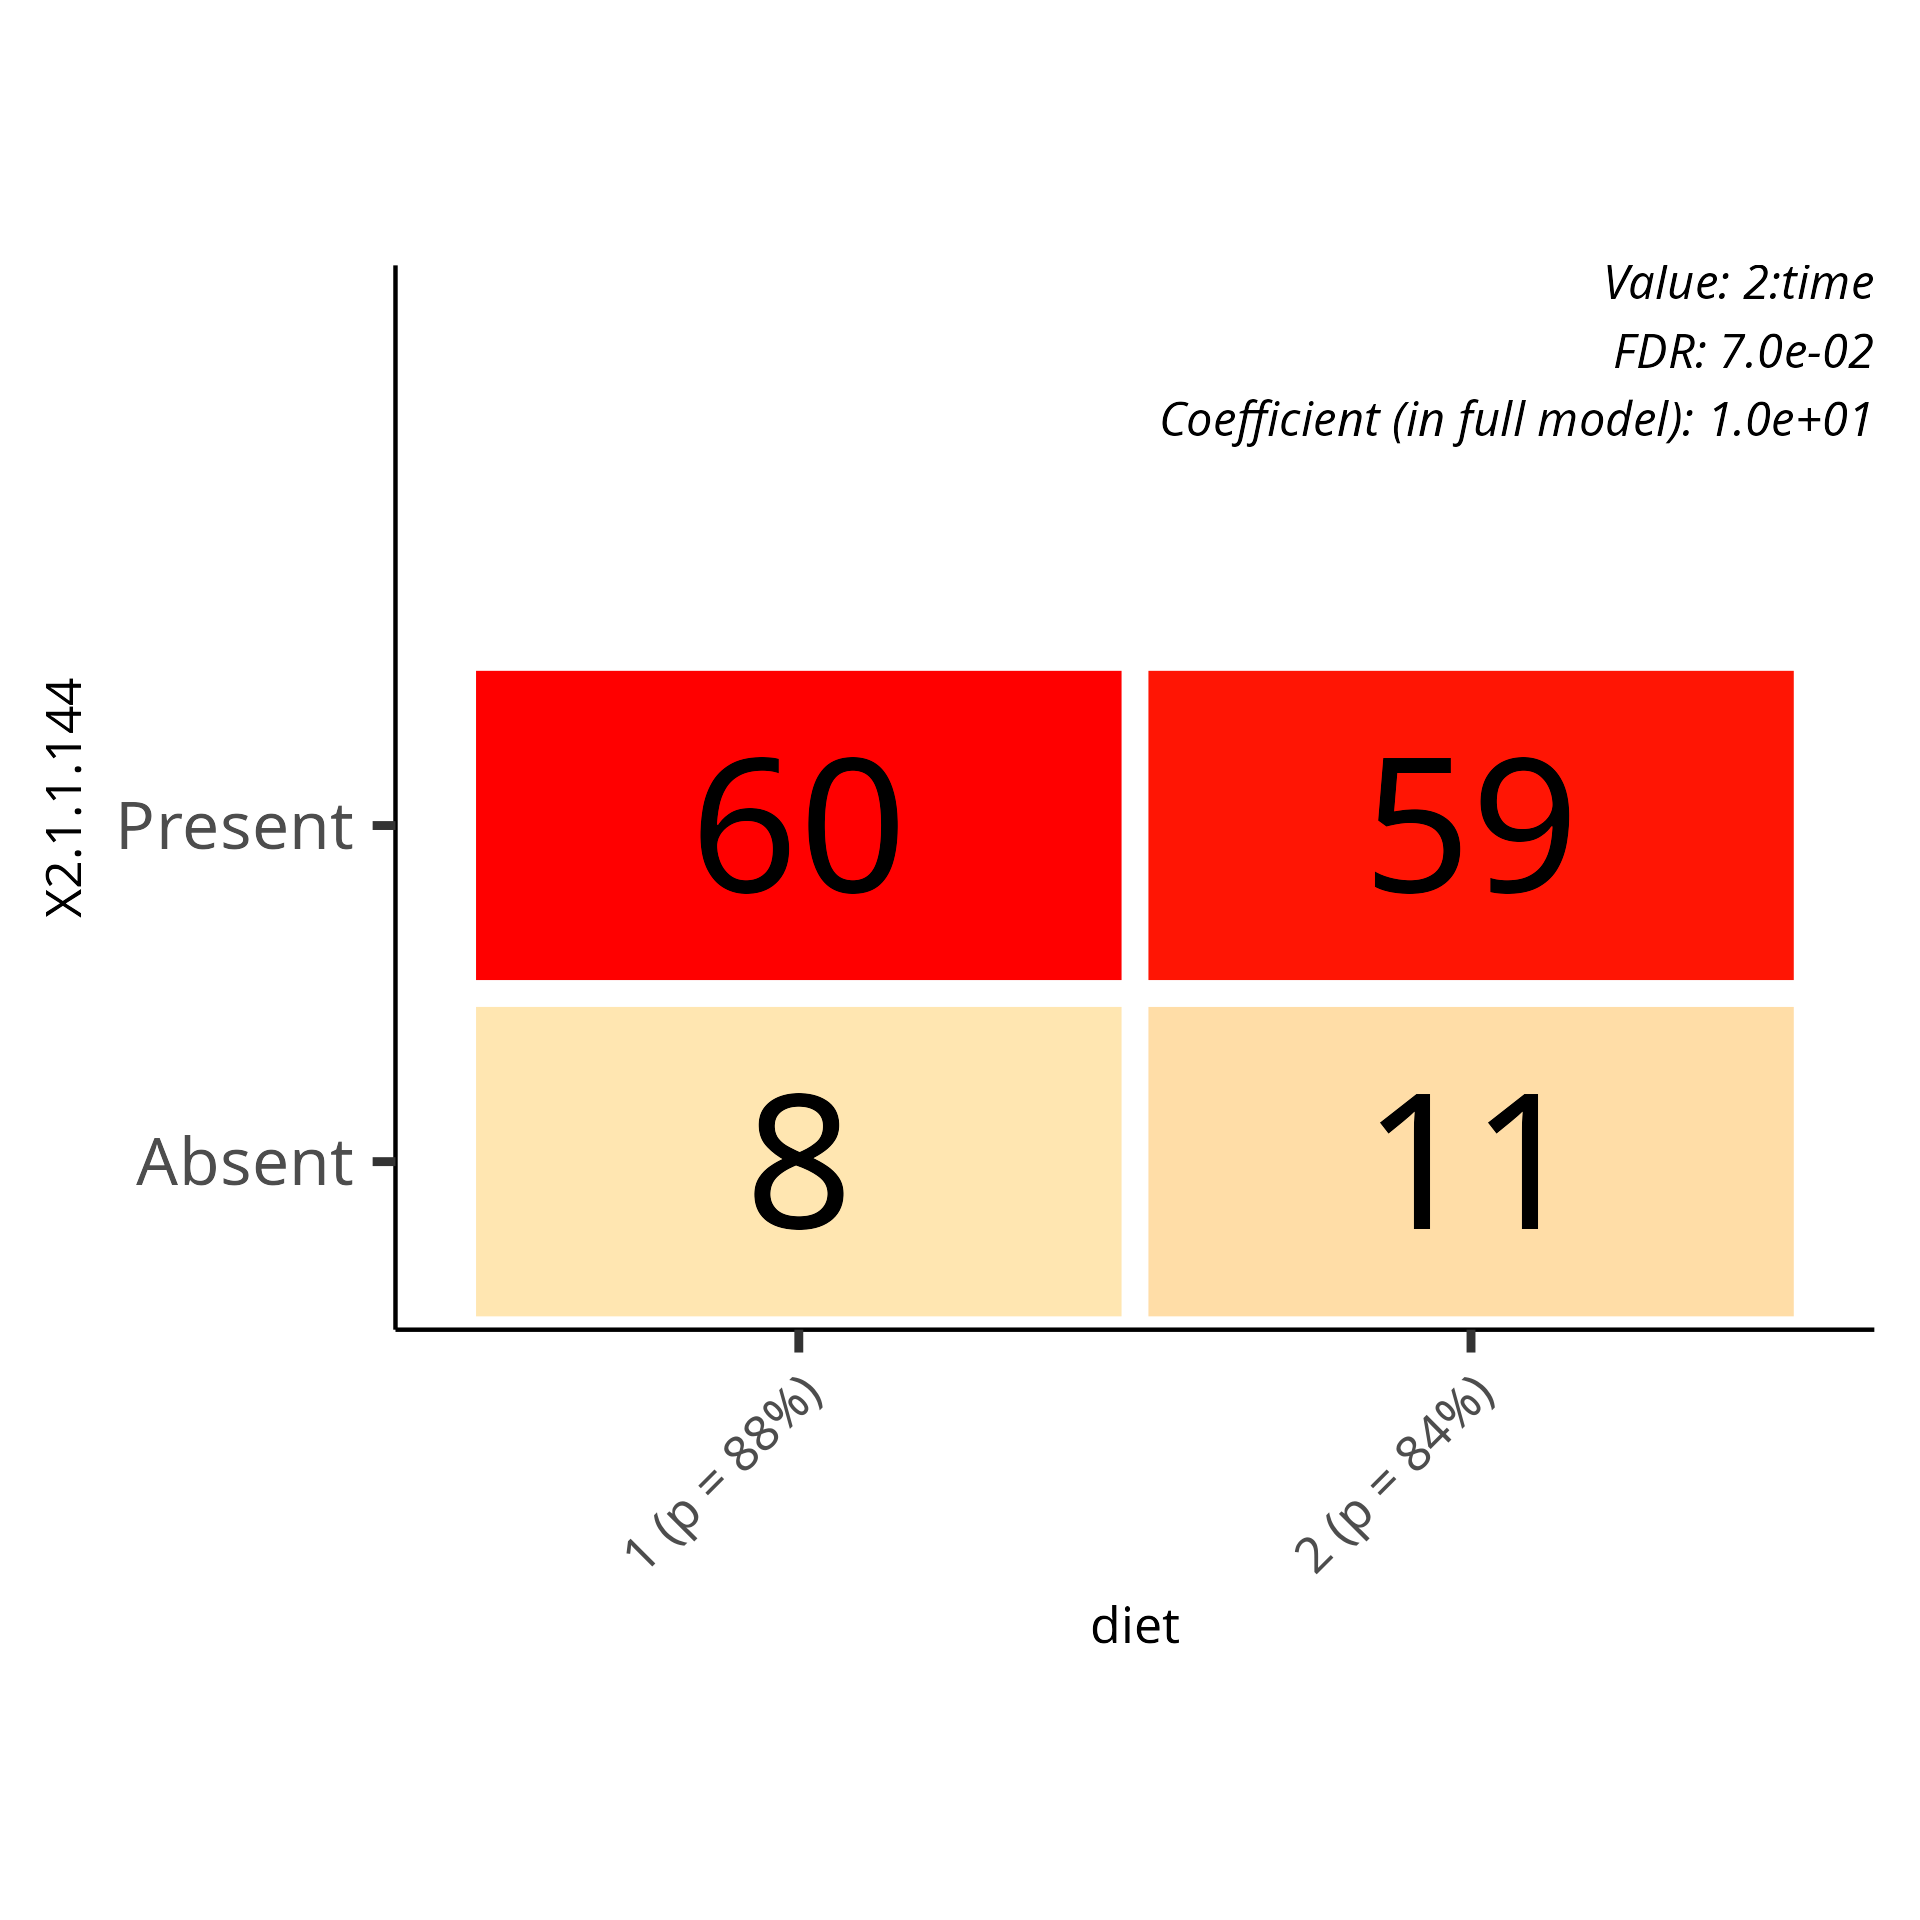
\includegraphics{../output/daa/daa_mtc/figures/association_plots/diet/logistic/diet_X2.1.1.144_logistic.png}\\
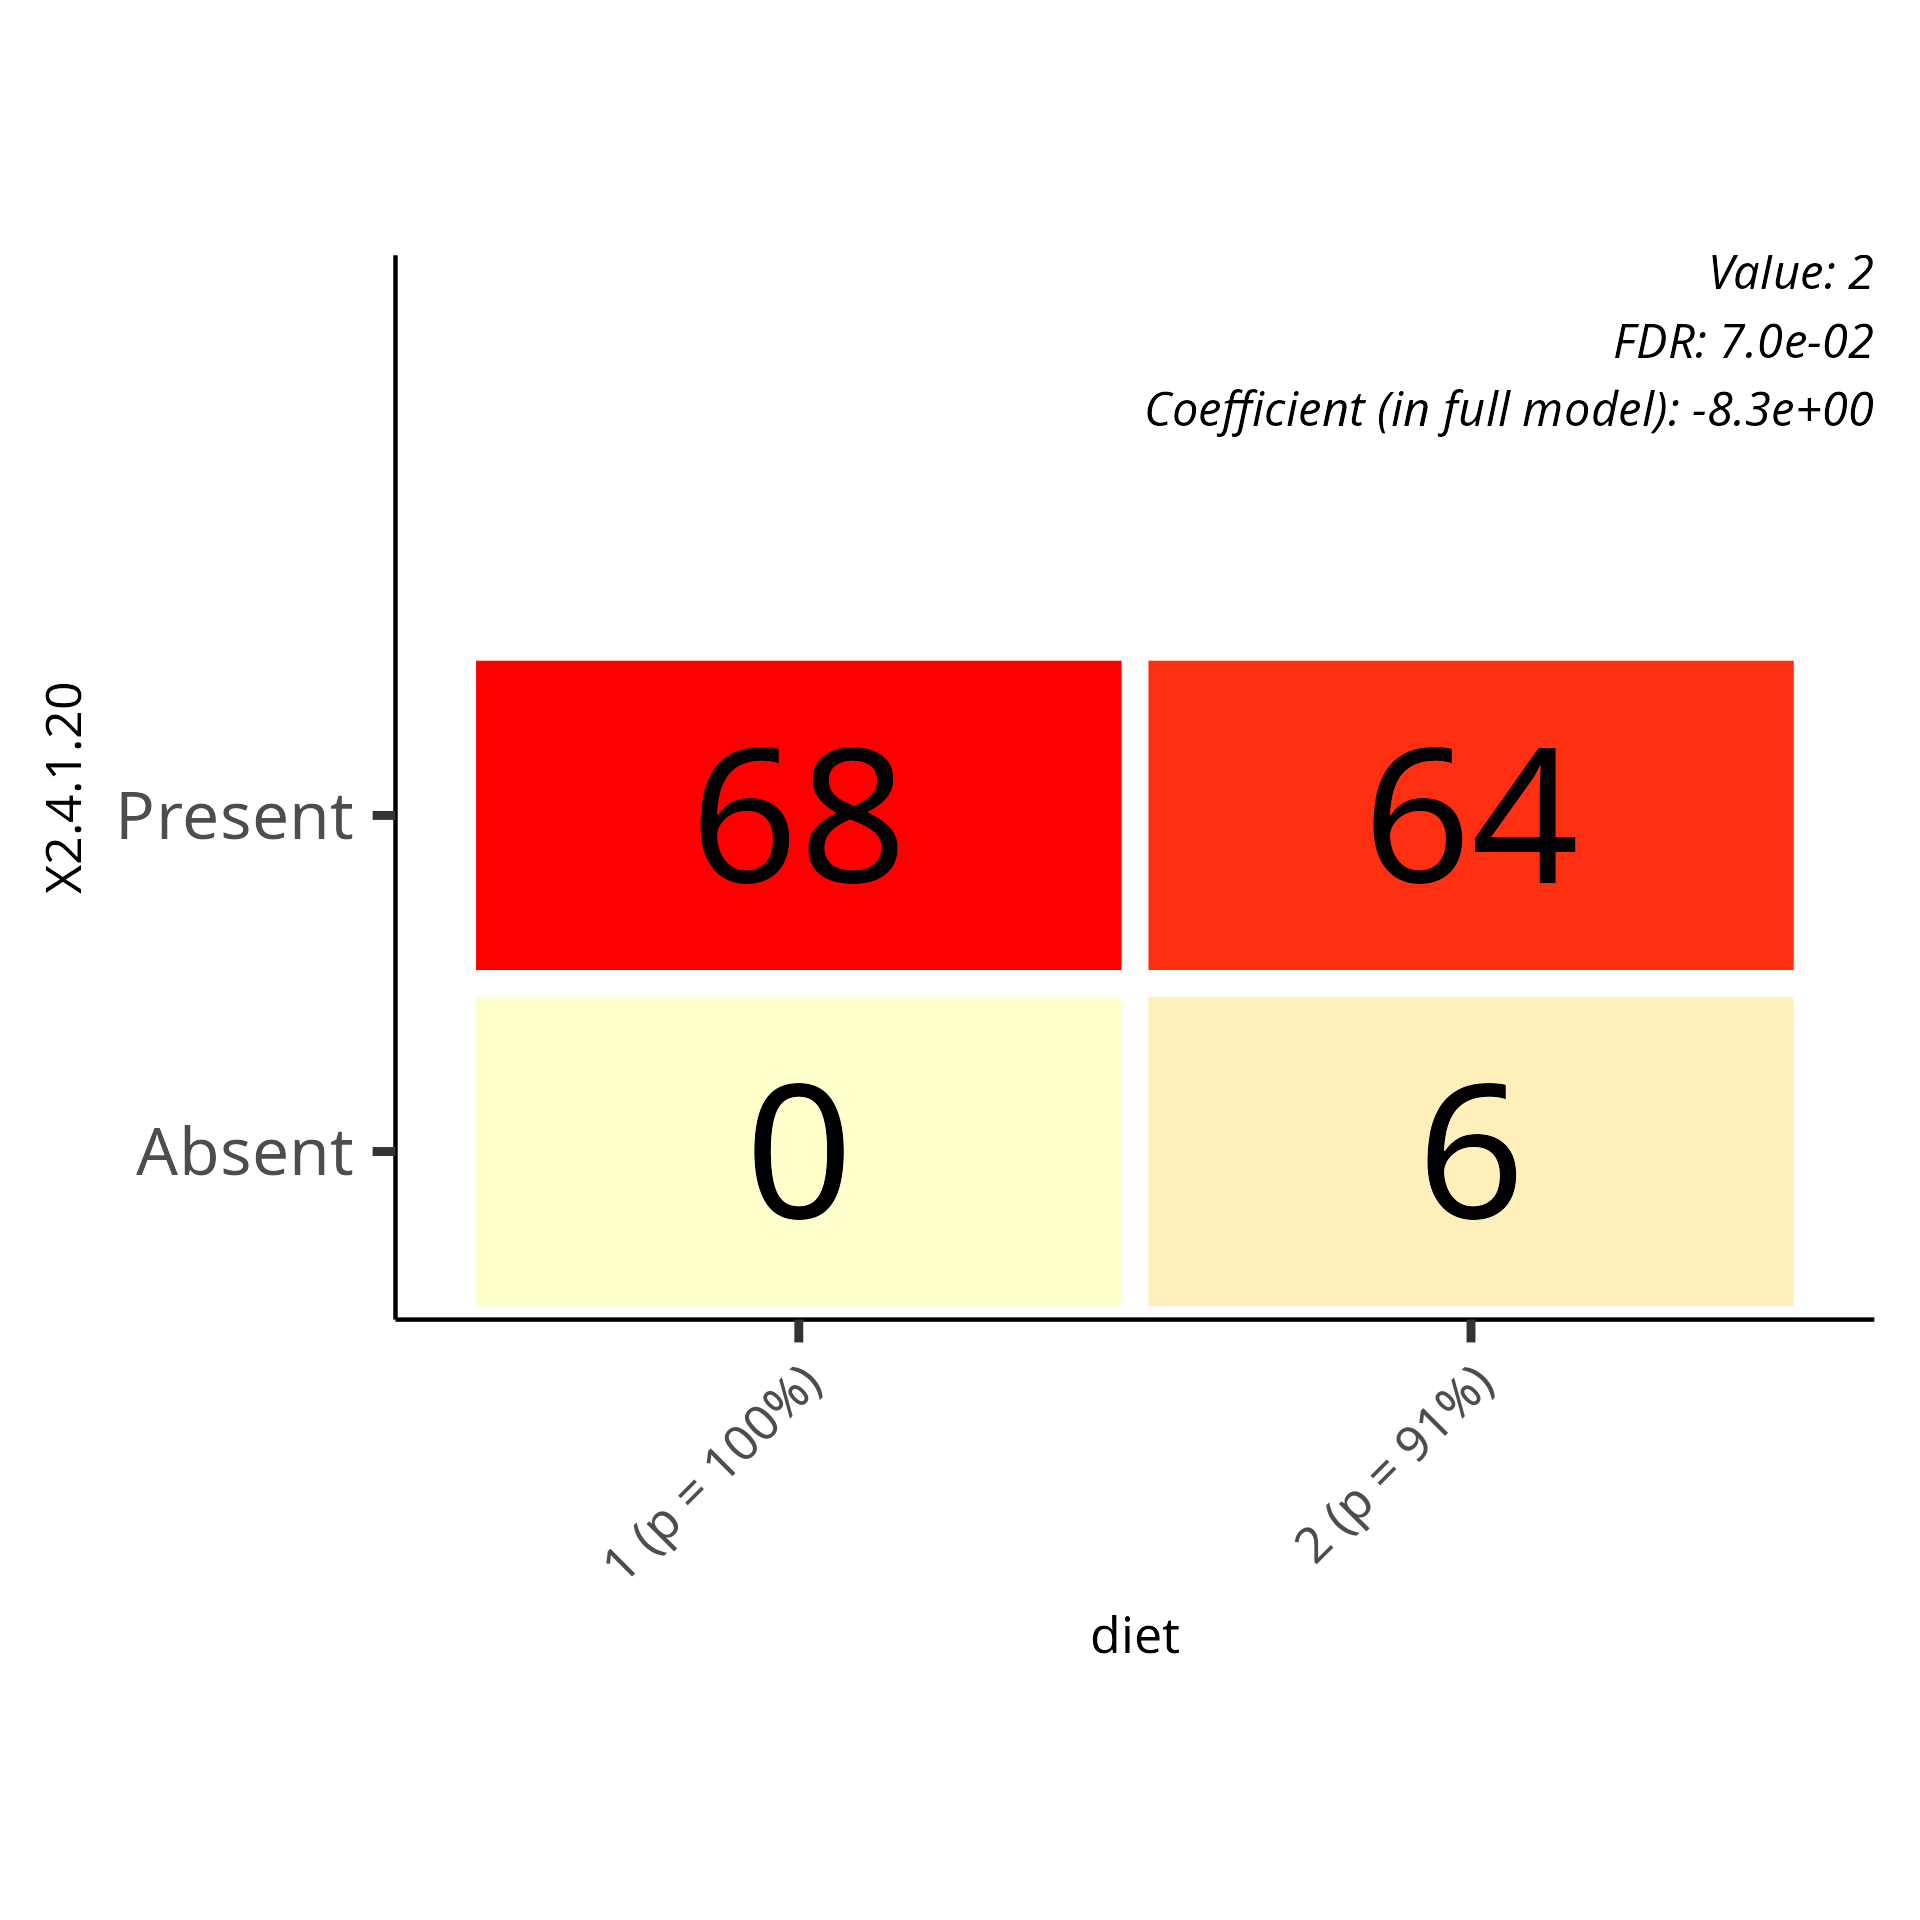
\includegraphics{../output/daa/daa_mtc/figures/association_plots/diet/logistic/diet_X2.4.1.20_logistic.png}\\
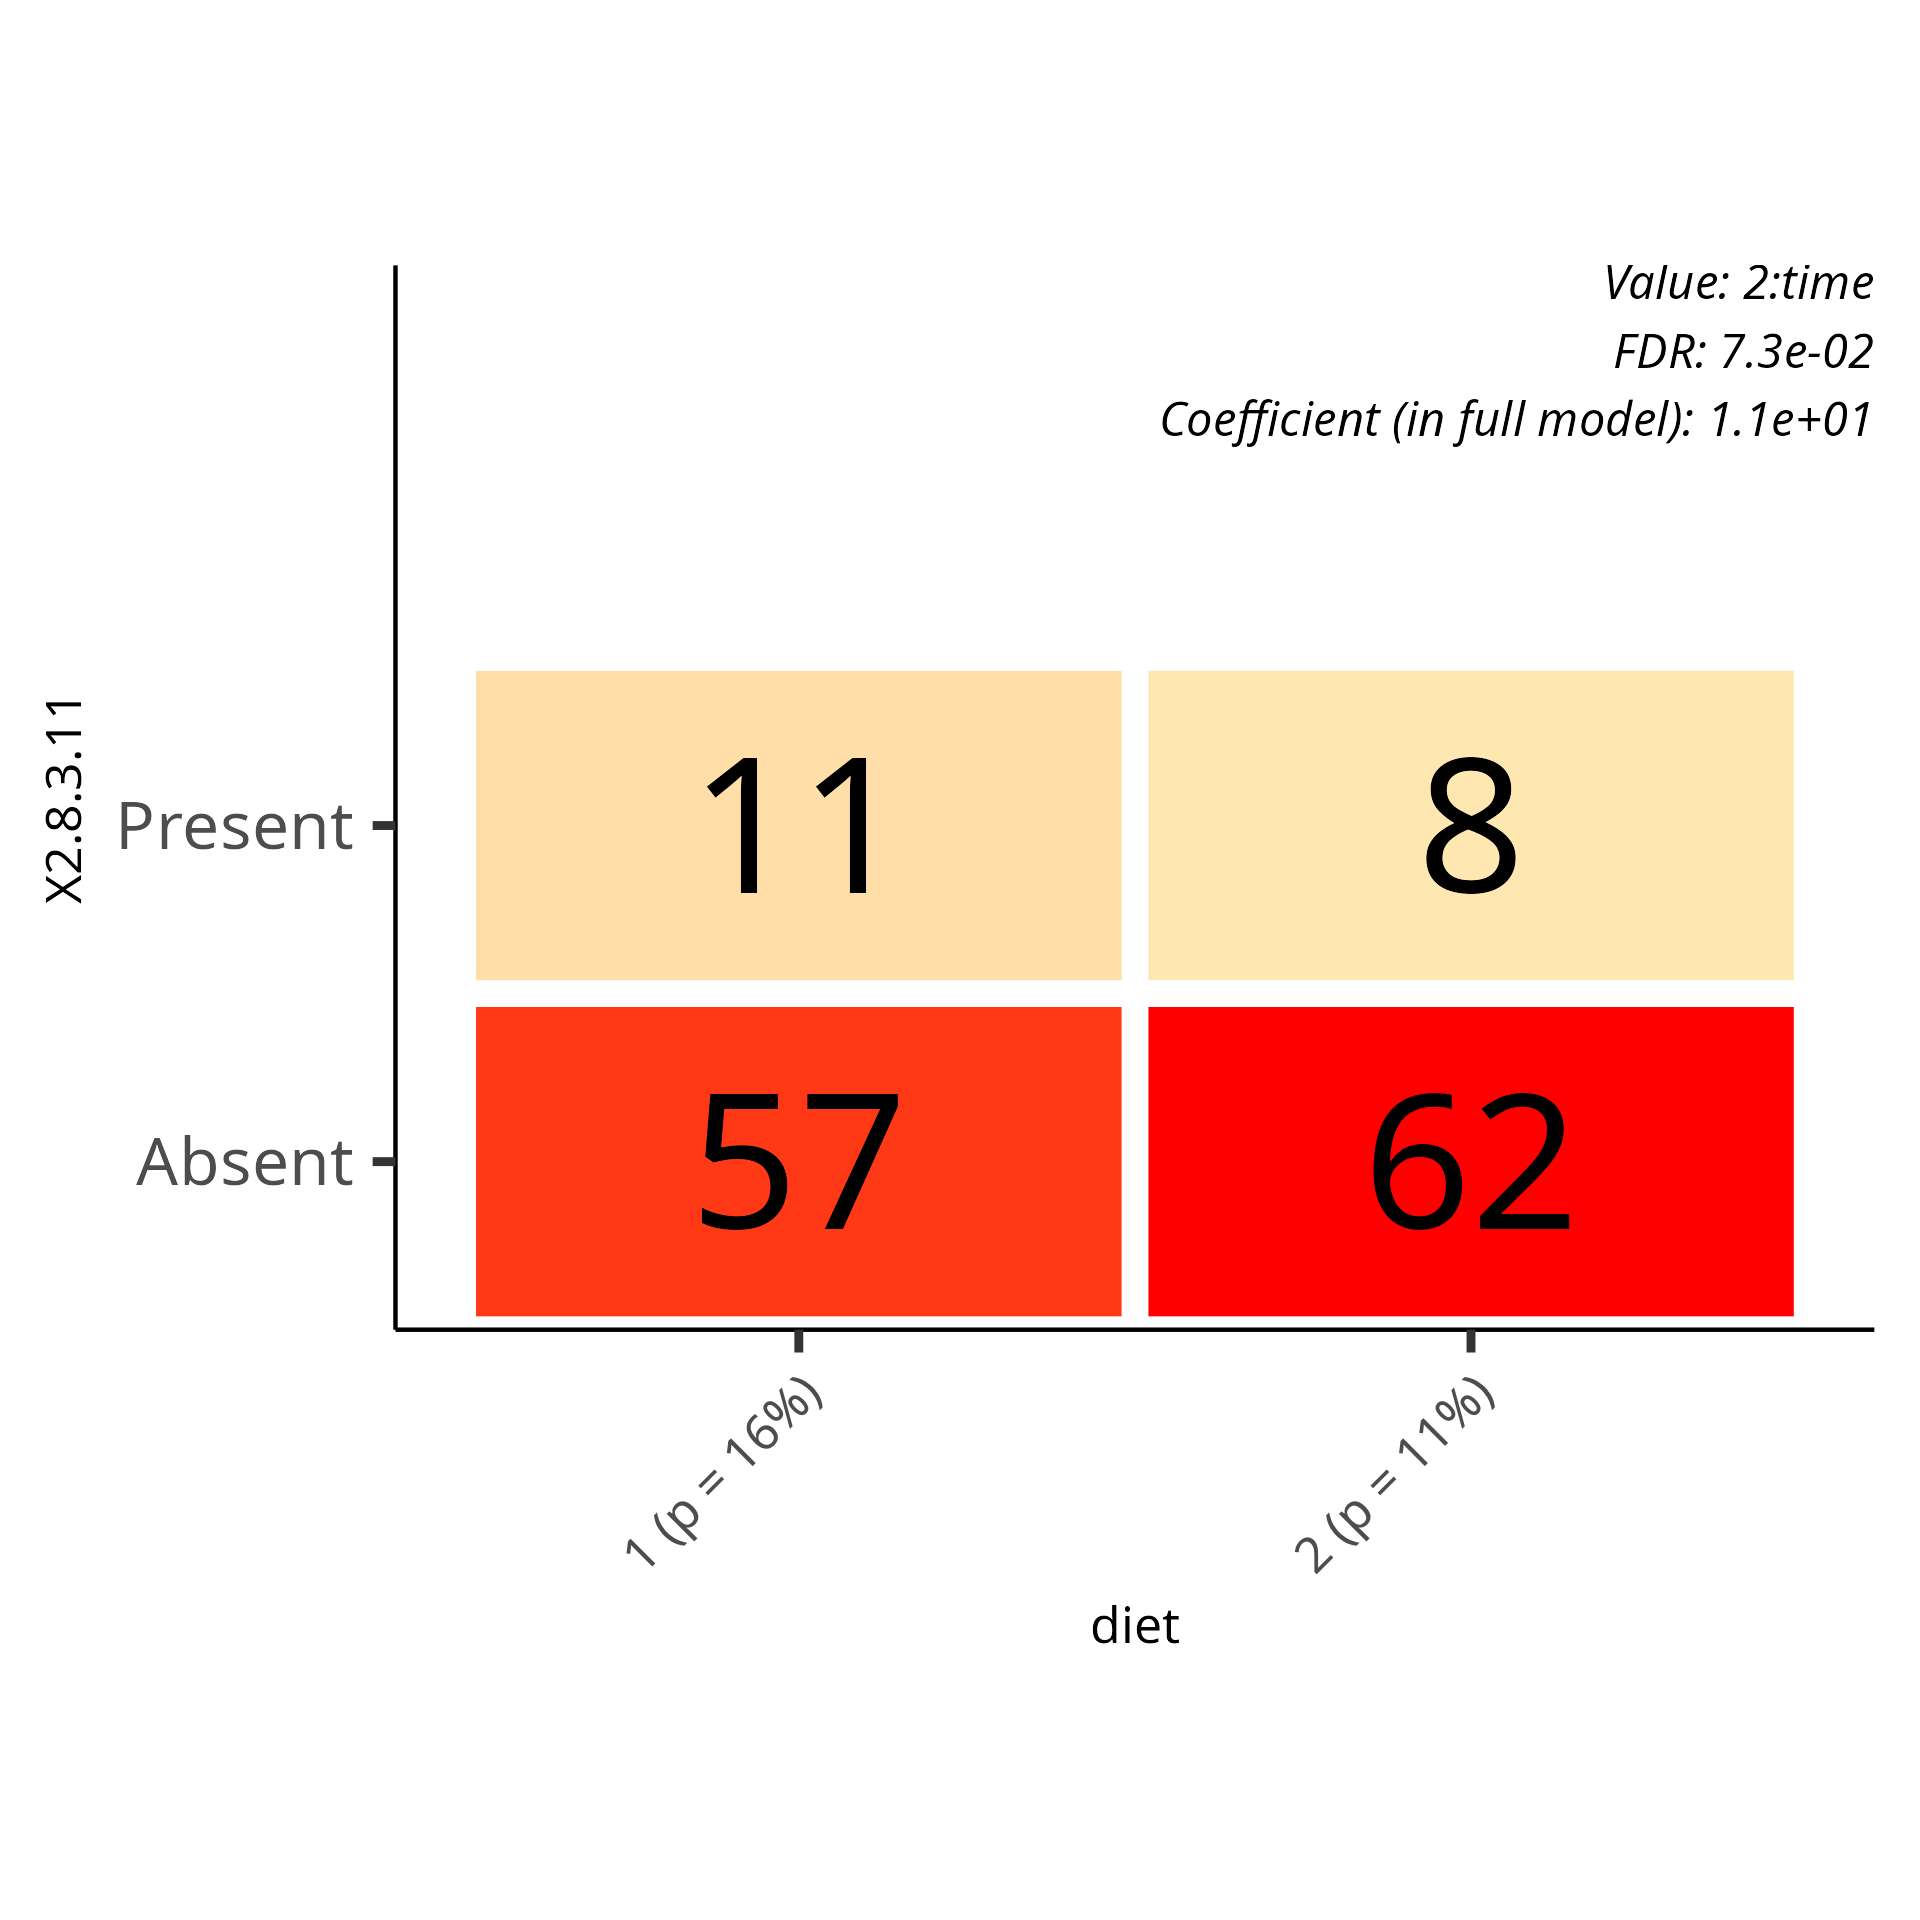
\includegraphics{../output/daa/daa_mtc/figures/association_plots/diet/logistic/diet_X2.8.3.11_logistic.png}\\
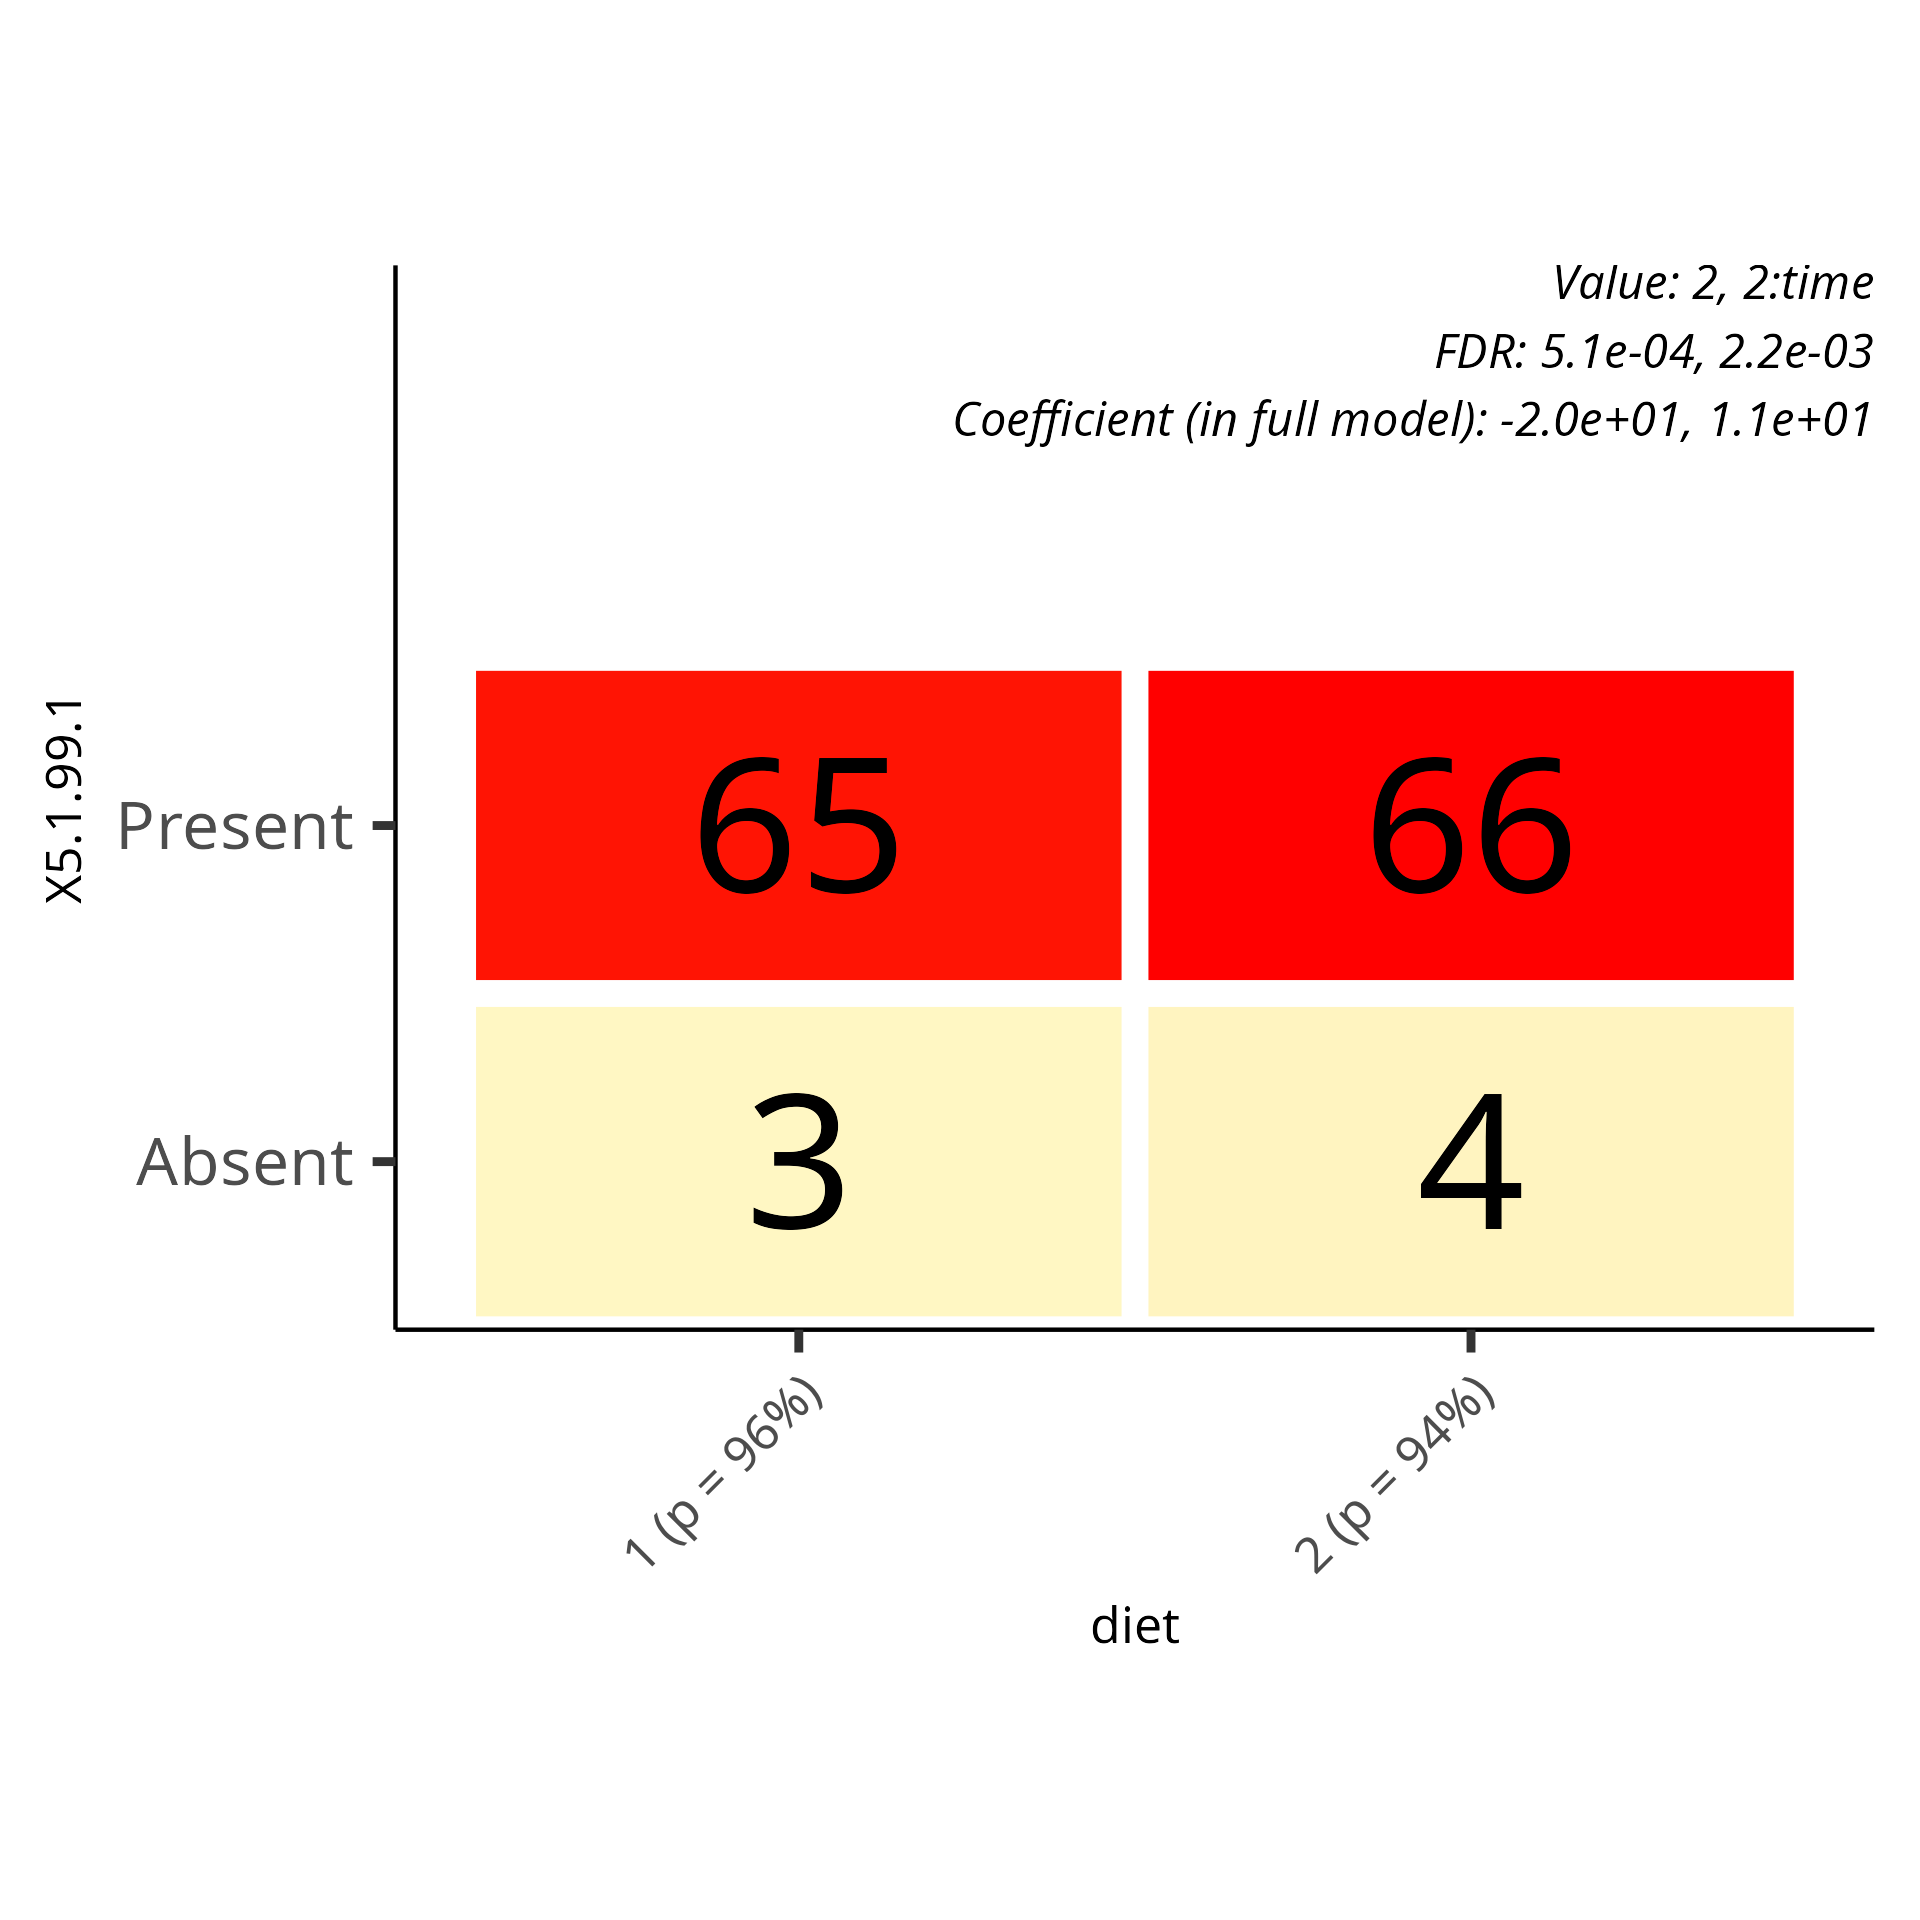
\includegraphics{../output/daa/daa_mtc/figures/association_plots/diet/logistic/diet_X5.1.99.1_logistic.png}\\
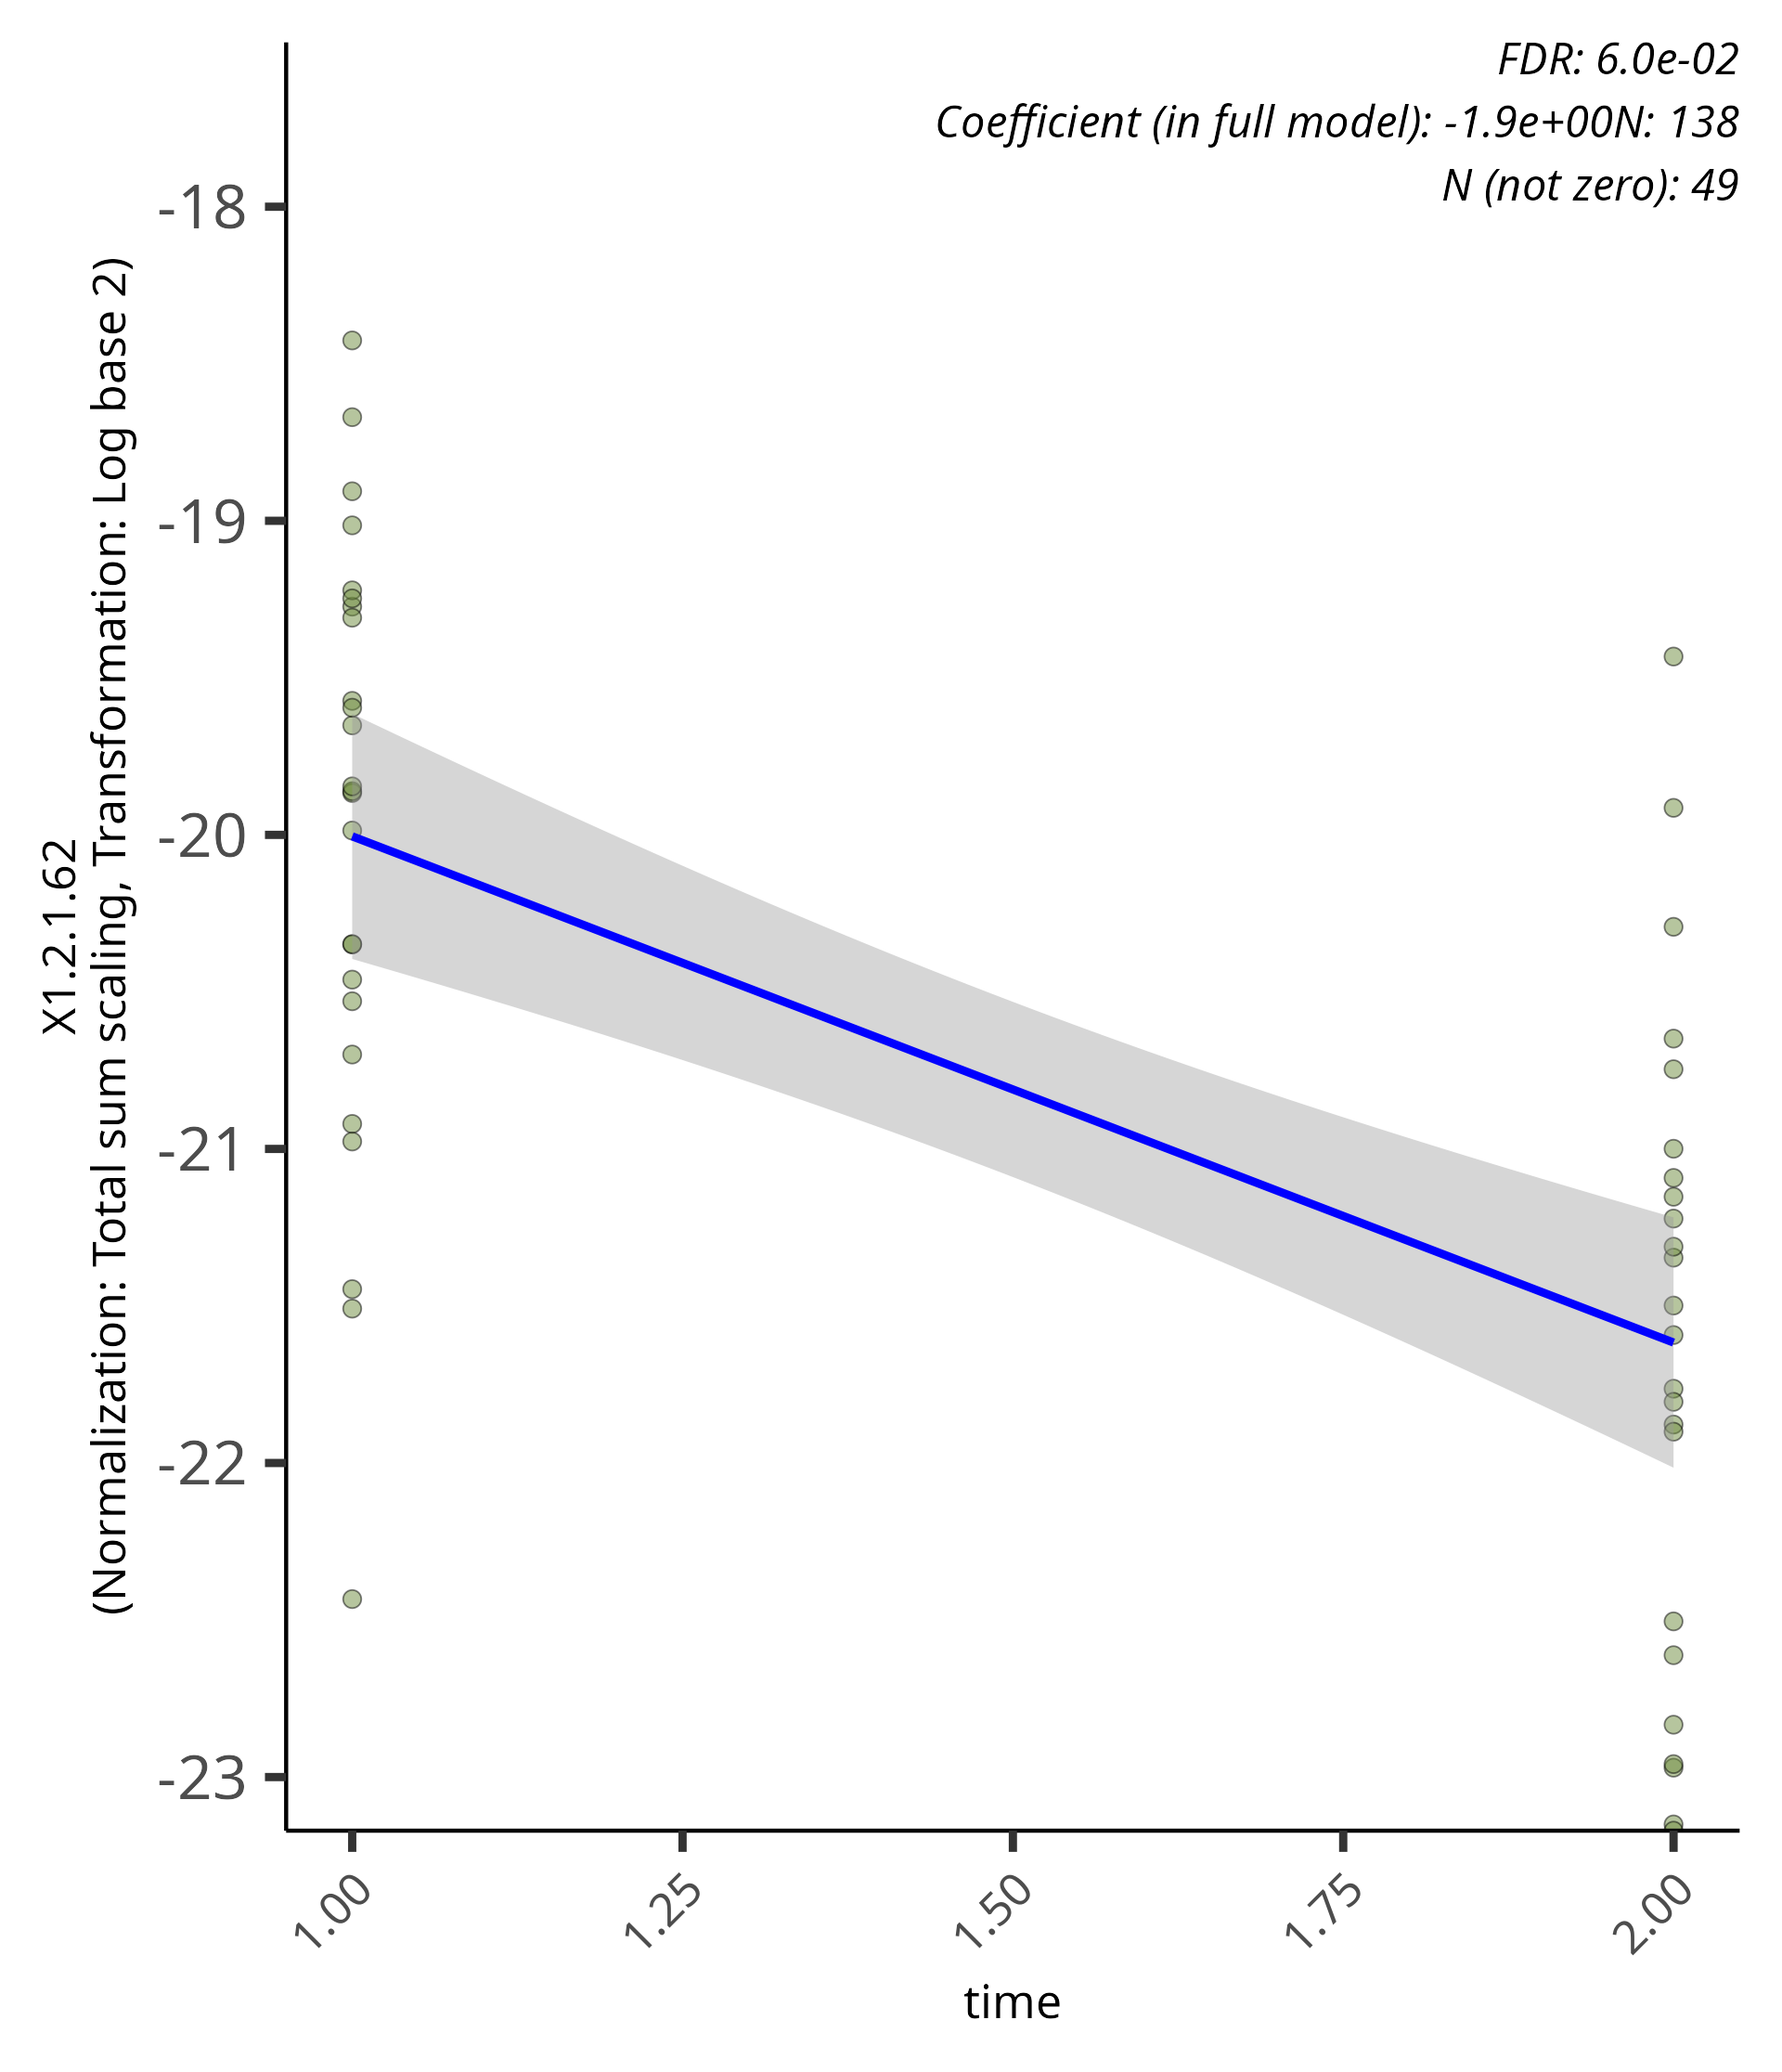
\includegraphics{../output/daa/daa_mtc/figures/association_plots/time/linear/time_X1.2.1.62_linear.png}\\
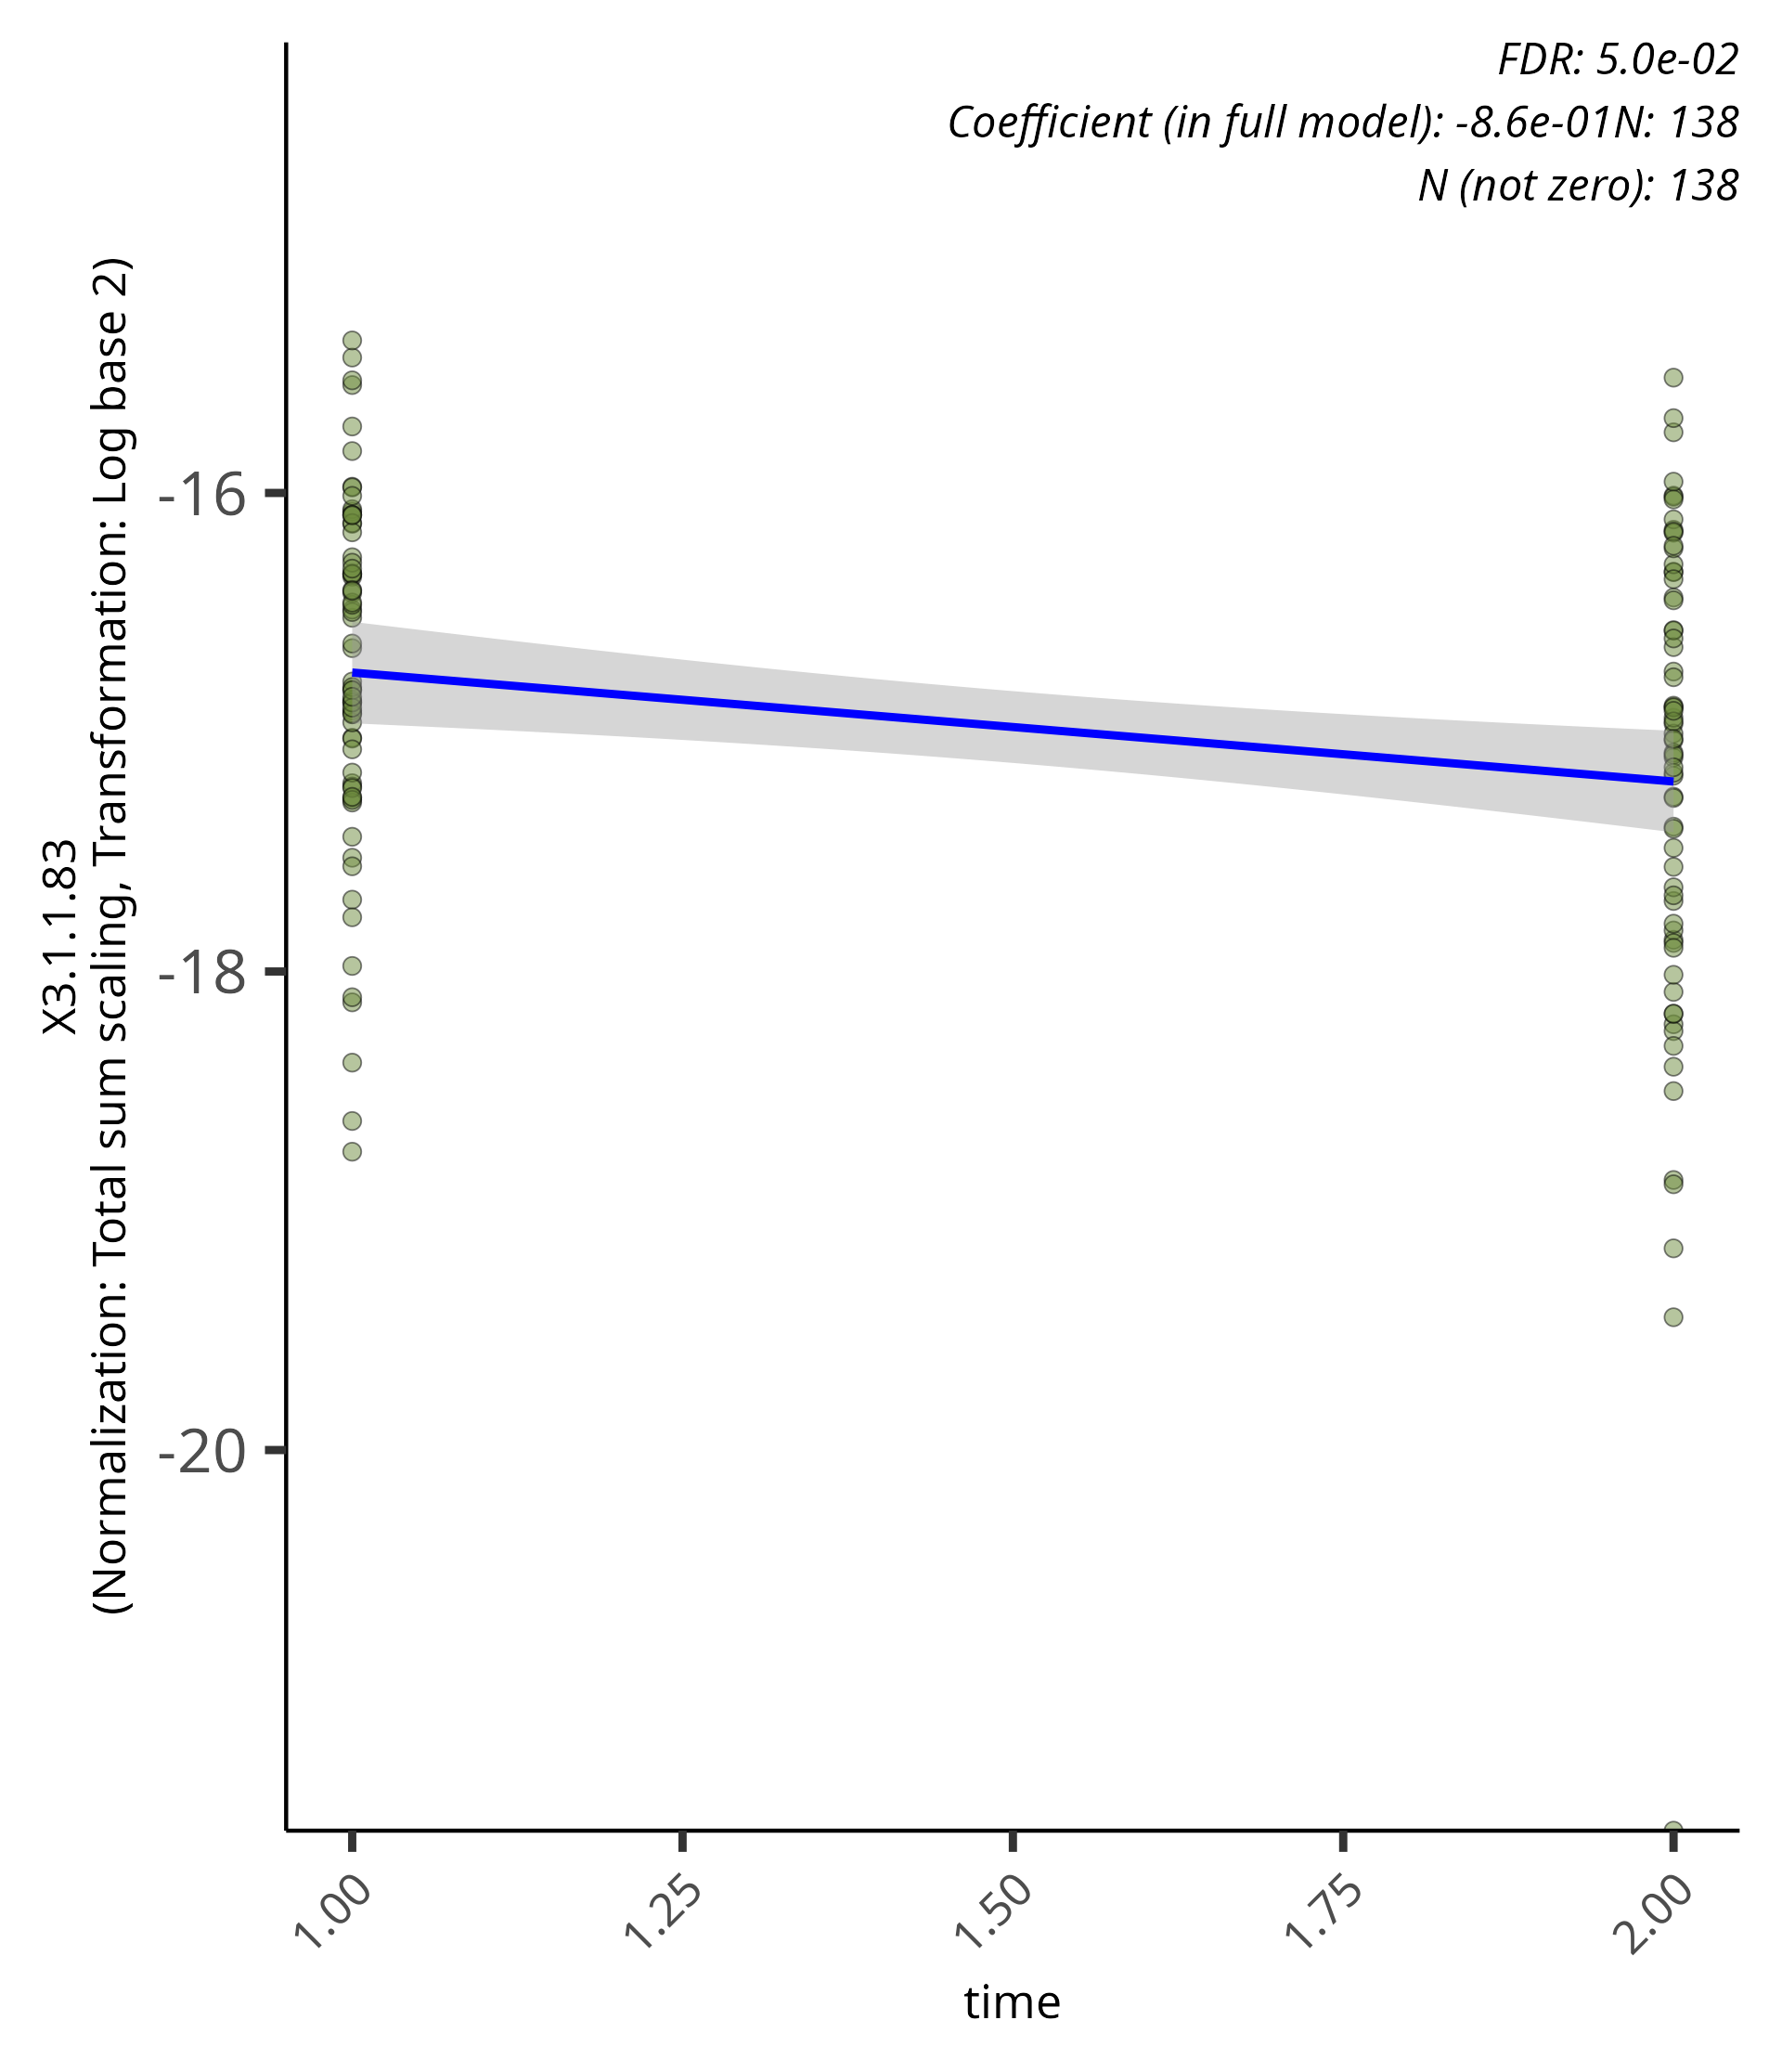
\includegraphics{../output/daa/daa_mtc/figures/association_plots/time/linear/time_X3.1.1.83_linear.png}\\
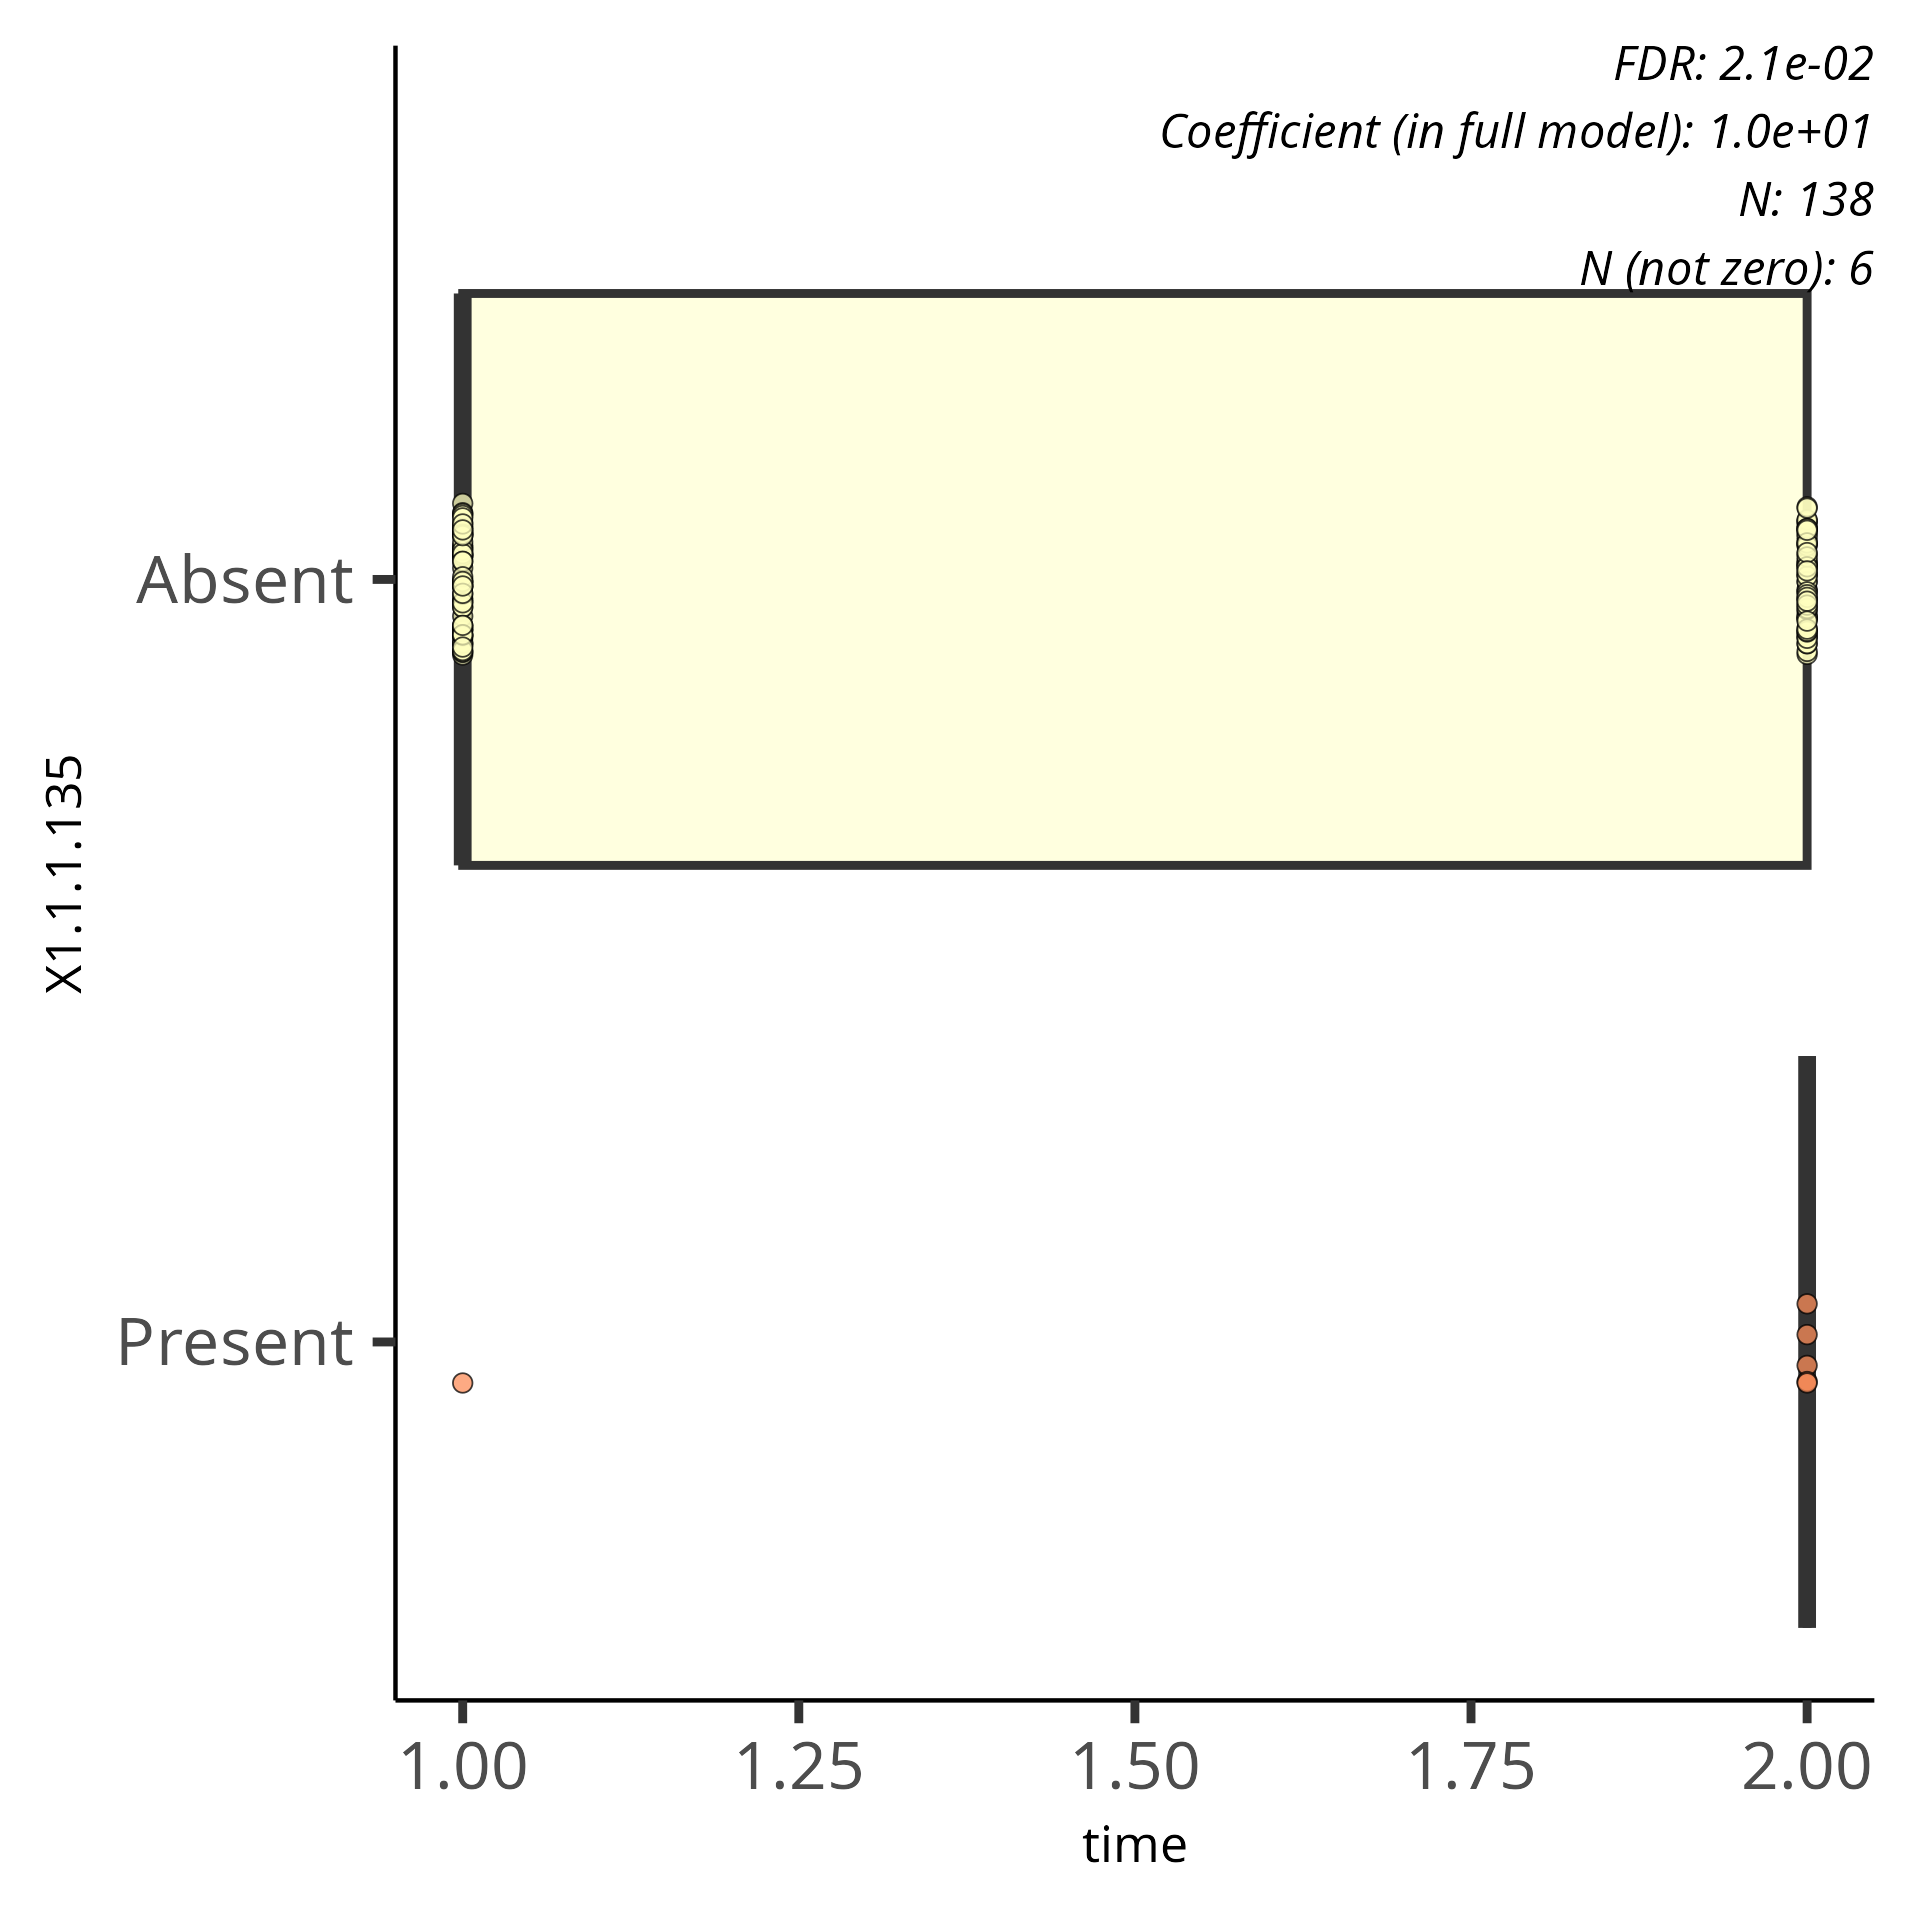
\includegraphics{../output/daa/daa_mtc/figures/association_plots/time/logistic/time_X1.1.1.135_logistic.png}\\
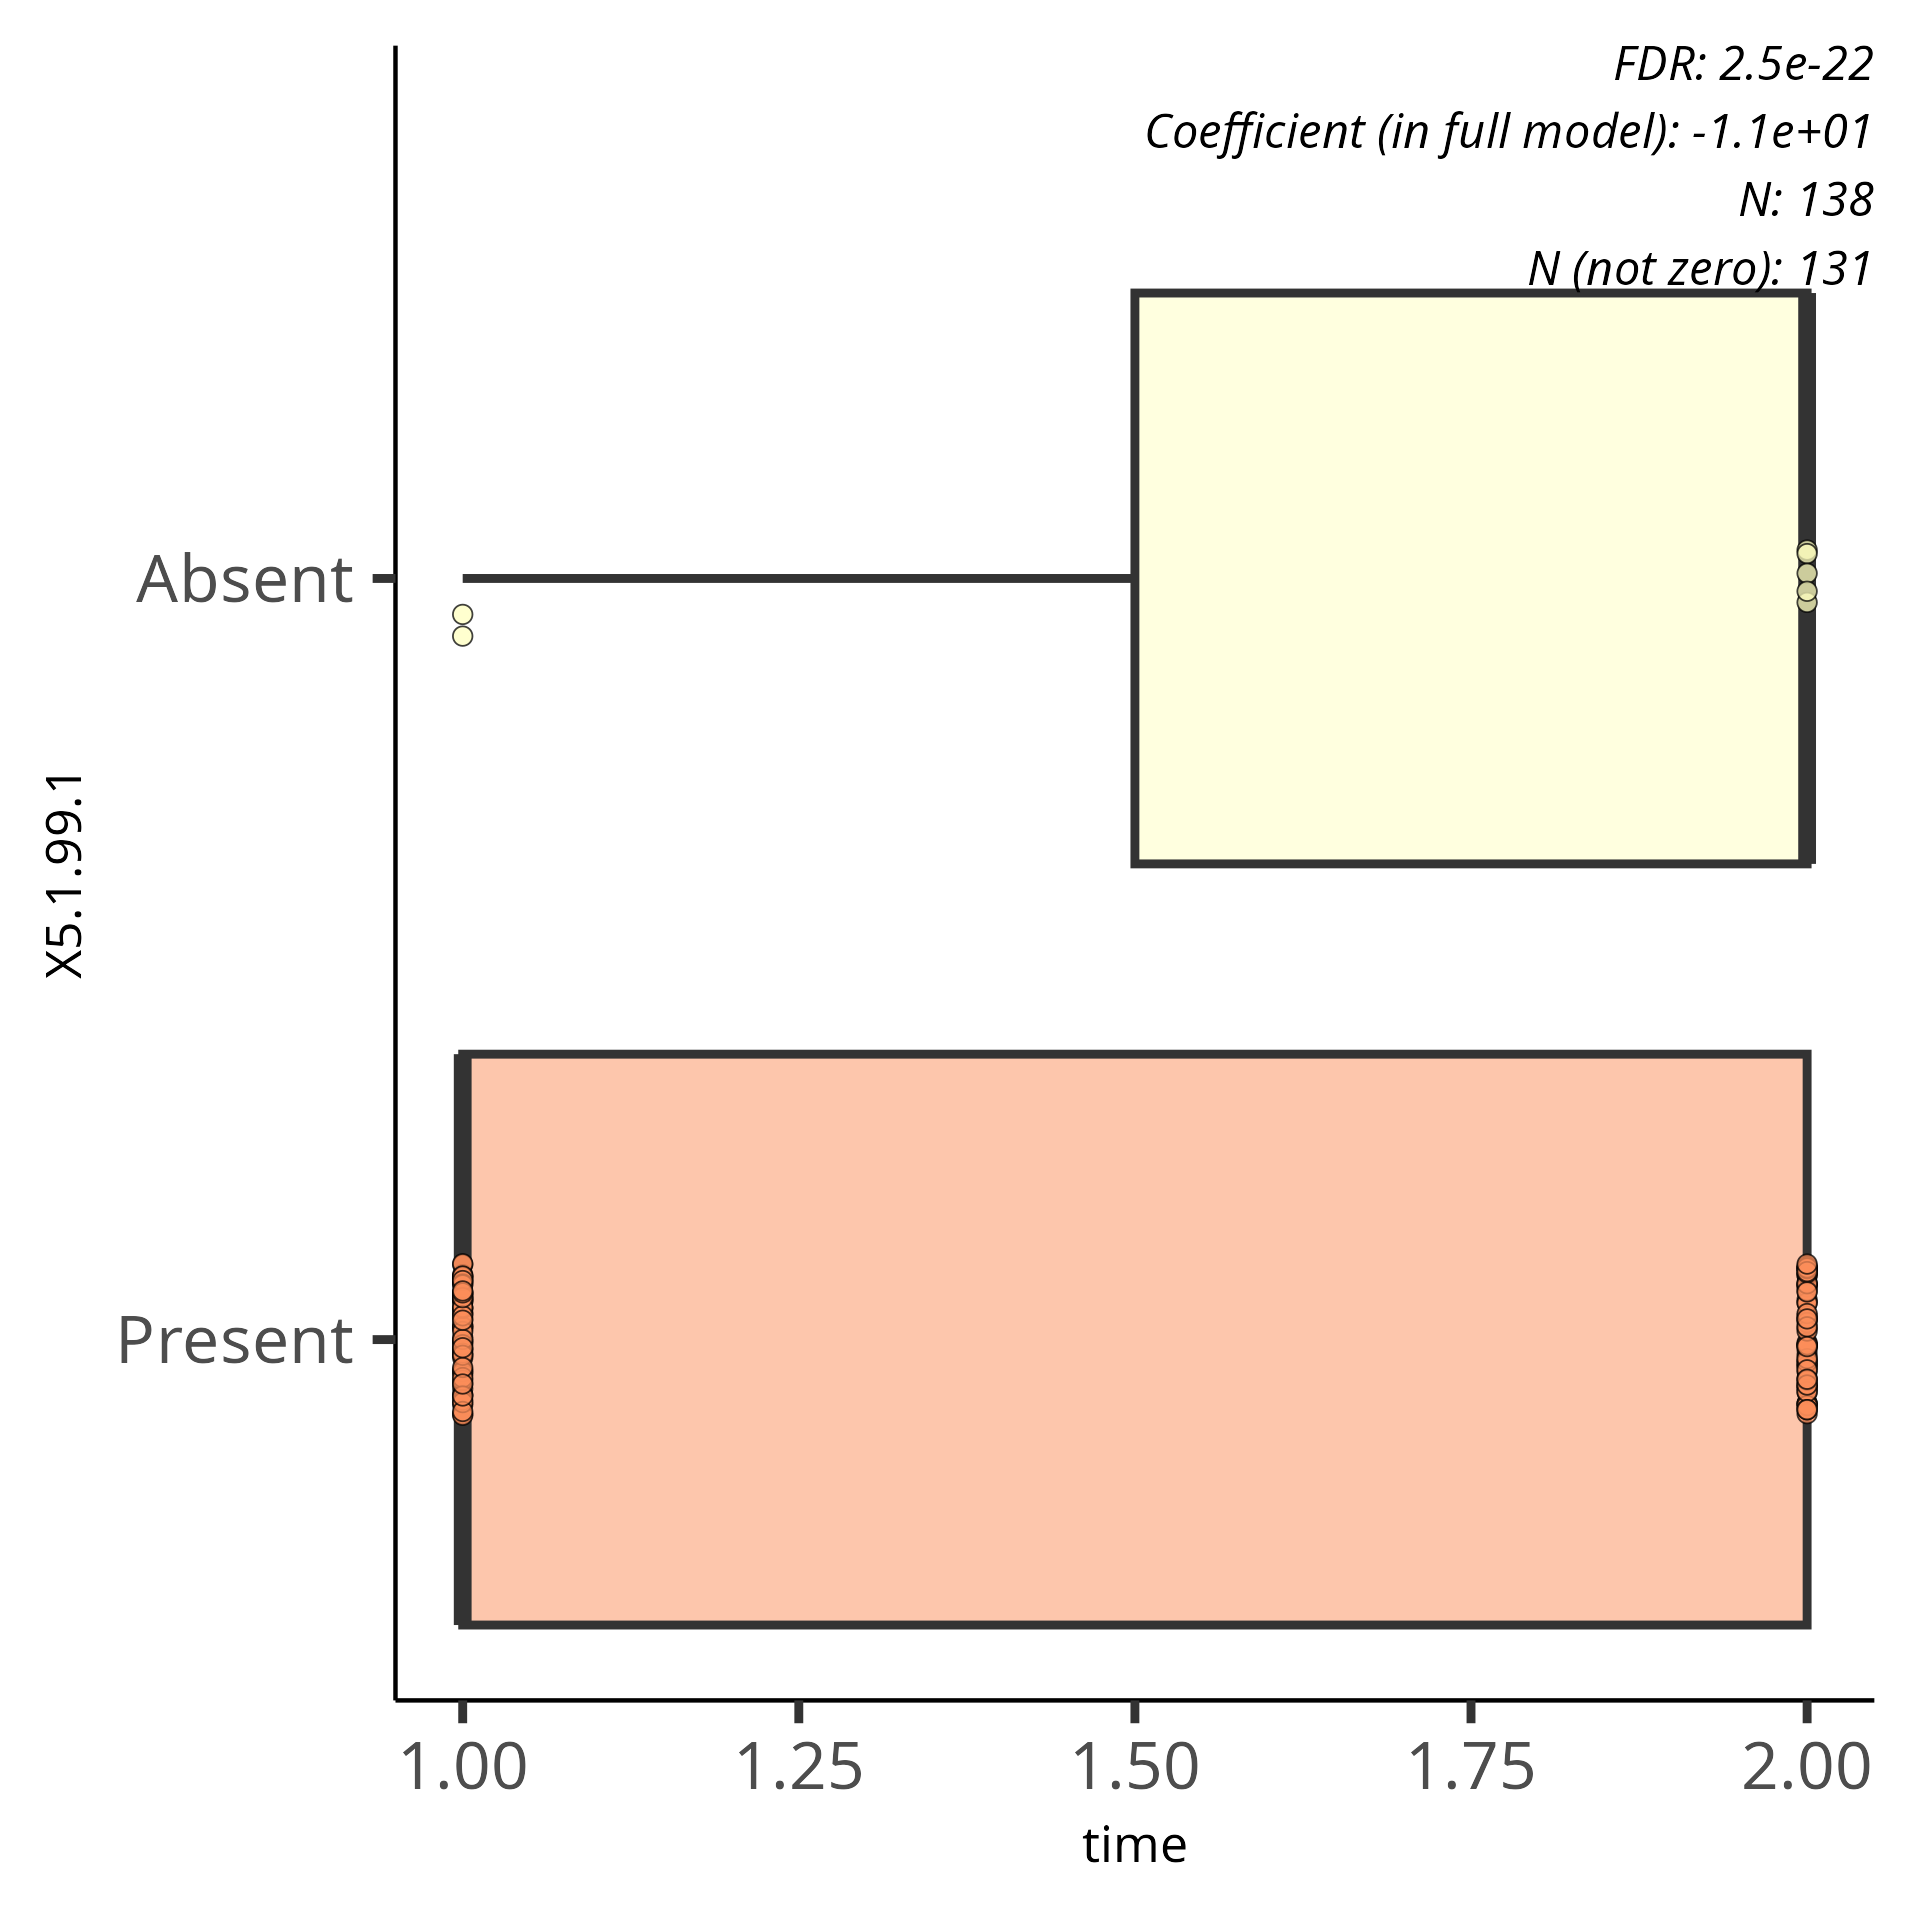
\includegraphics{../output/daa/daa_mtc/figures/association_plots/time/logistic/time_X5.1.99.1_logistic.png}




\end{document}
